\documentclass[12pt]{article}

\usepackage{sbc-template}
\usepackage{graphicx}
\usepackage[brazilian]{babel}
\usepackage[utf8]{inputenc}
\usepackage[T1]{fontenc}
\usepackage{lmodern}
\usepackage{float}
\usepackage{subcaption}
\usepackage{indentfirst}
\usepackage{amsmath}

\sloppy

\title{Manual de Uso Básico da Calculadora Científica Casio FX-82MS}

\author{Beatriz Regina Nahas¹}
\address{Instituto Federal do Paraná -- Campus Pinhais
\email{beatriz.nahas@gmail.com}}

\begin{document}

\maketitle

\begin{resumo}
    Este manual apresenta as principais funções da calculadora científica Casio FX-82MS 
    voltadas ao estudo de Estatística, com foco em estudantes recém-ingressados 
    em cursos da área de Tecnologia da Informação. O objetivo é promover a autonomia no uso da 
    ferramenta como recurso de apoio à resolução e à interpretação de problemas estatísticos,
    abordando desde operações aritméticas básicas e potências até recursos de memória, 
    cálculos estatísticos e resolução de erros comuns. Os exemplos apresentados são 
    contextualizados com conteúdos da disciplina de Probabilidade e Estatística do curso de
    Bacharelado em Ciência da Computação do Instituto Federal do Paraná (IFPR) -- Campus Pinhais.
\end{resumo}

\section{Introdução}

A calculadora científica constitui uma ferramenta de apoio relevante
para estudantes de cursos da área de Ciências Exatas, especialmente em
disciplinas que envolvem a realização e a interpretação de cálculos
matemáticos. No estudo de Estatística, sua utilização pode auxiliar na
execução de cálculos repetitivos e na obtenção de resultados numéricos,
permitindo que o estudante concentre maior atenção na compreensão dos
procedimentos e na interpretação dos resultados. Apesar disso, muitos
estudantes ingressam no ensino superior sem familiaridade com os recursos
e as funcionalidades desse tipo de equipamento, o que pode dificultar sua
utilização adequada durante as atividades acadêmicas.

A utilização de recursos tecnológicos como instrumentos de apoio ao
ensino e à aprendizagem da Matemática tem sido discutida no campo da
Educação Matemática. Borba e Penteado \cite{borba2019} destacam que a
incorporação de recursos tecnológicos ao processo educacional está
relacionada às formas pelas quais professores e estudantes interagem com
o conhecimento. De maneira complementar, Pillon et al. \cite{pillon2020}
identificam, em revisão integrativa, diferentes recursos e abordagens
digitais empregados no ensino-aprendizagem de Matemática. A elaboração
de materiais voltados especificamente ao uso de calculadoras também
encontra precedentes: Becker et al. \cite{becker2020} apresentam um
minicurso de calculadora científica desenvolvido no contexto da formação
em Matemática no Instituto Federal do Rio Grande do Sul (IFRS), o que
reforça a pertinência de iniciativas dessa natureza.

Nesse contexto, este manual apresenta uma introdução ao uso da
calculadora científica Casio FX-82MS \cite{casio2004}, com foco em sua
aplicação no estudo de Estatística e destinado principalmente a
estudantes recém-ingressados em cursos da área de Tecnologia da
Informação. A escolha desse modelo está
relacionada à sua disponibilidade no mercado, à sua proposta voltada ao
público estudantil e à presença de recursos matemáticos e estatísticos
\cite{neubert2026}. As fórmulas, notações e organização dos exemplos
seguem a obra \textit{Estatística Fácil}, de Crespo \cite{crespo2009},
mantendo consistência com a disciplina de Probabilidade e Estatística
do curso Bacharelado em Ciência da Computação (IFPR -- Campus Pinhais) 
e estabelecendo relação direta entre a formulação matemática
dos problemas e sua aplicação prática por meio da calculadora.

O objetivo é promover a autonomia dos estudantes no uso da calculadora,
apresentando seus recursos de maneira gradual e contextualizada, com
exemplos que relacionam os procedimentos realizados na calculadora aos
conceitos matemáticos envolvidos. A calculadora é apresentada como
ferramenta de apoio à resolução dos problemas, e não como substituta da
compreensão dos conceitos estatísticos.

\section{Conhecendo a Calculadora}

A Casio FX-82MS é uma calculadora científica não programável, equipada com visor de duas linhas e recursos destinados à realização de cálculos matemáticos e estatísticos. O modelo possui 240 funções, memória para nove variáveis, memória independente e recursos estatísticos, incluindo editor de dados, cálculo de desvio padrão e análise de regressão \cite{casio2004}. A alimentação é realizada por uma pilha do tipo AAA, e o equipamento possui recurso de desligamento automático para economia de energia.

\subsection{Primeira e Segunda Edição}

A segunda edição da FX-82MS representa uma atualização da linha MS com modificações principalmente relacionadas ao design, à ergonomia e à facilidade de utilização. Segundo a Casio, o projeto da segunda edição buscou proporcionar maior conforto durante o uso, melhorar a legibilidade das teclas e facilitar a identificação e o acionamento dos comandos. Entre as alterações destacadas pela fabricante estão o corpo mais arredondado, a ampliação de teclas numéricas e a utilização de caracteres mais legíveis, além de modificações na disposição e na identificação visual de algumas teclas.

\begin{figure}[H]
    \centering
    \begin{subfigure}{0.35\textwidth}
        \centering
        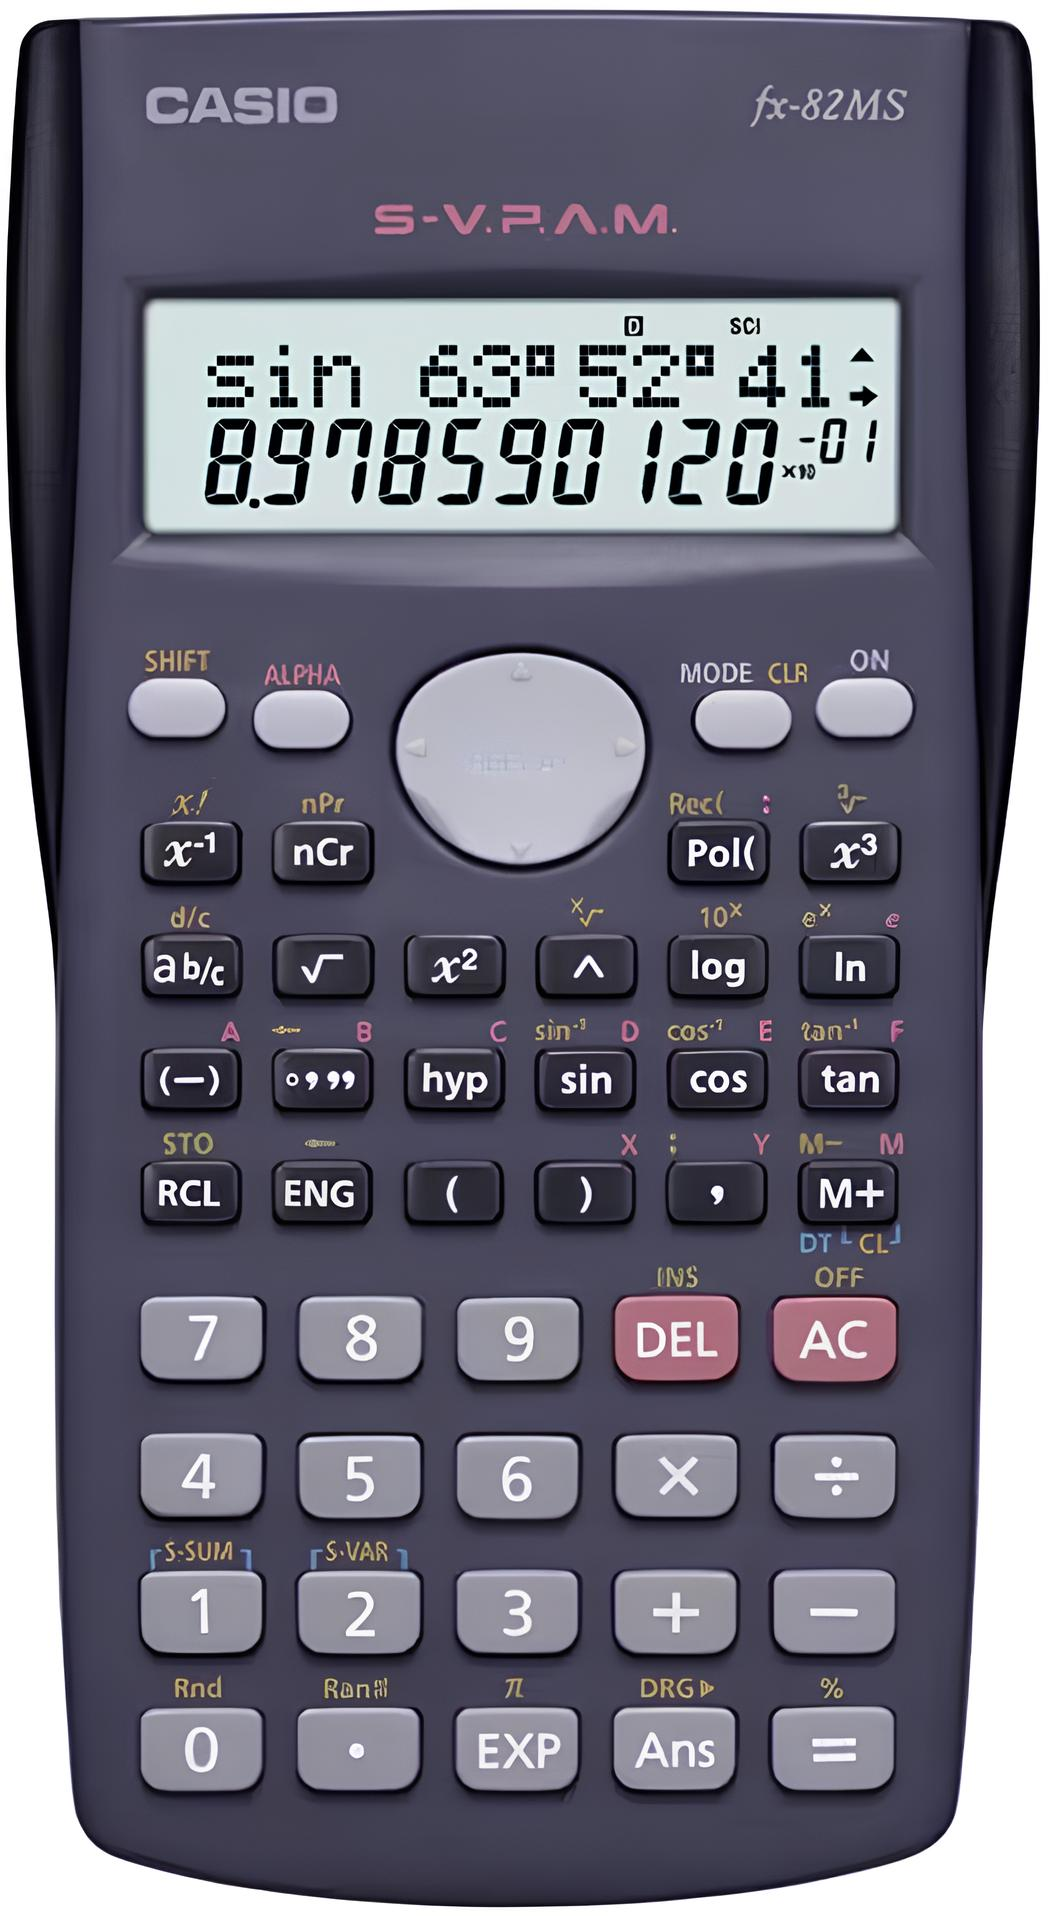
\includegraphics[width=0.66\textwidth]{img/casio-1ed.jpg}
        \caption{1\textsuperscript{a} Edição}
        \label{fig:ed1}
    \end{subfigure}
    %\hfill
    \begin{subfigure}{0.35\textwidth}
        \centering
        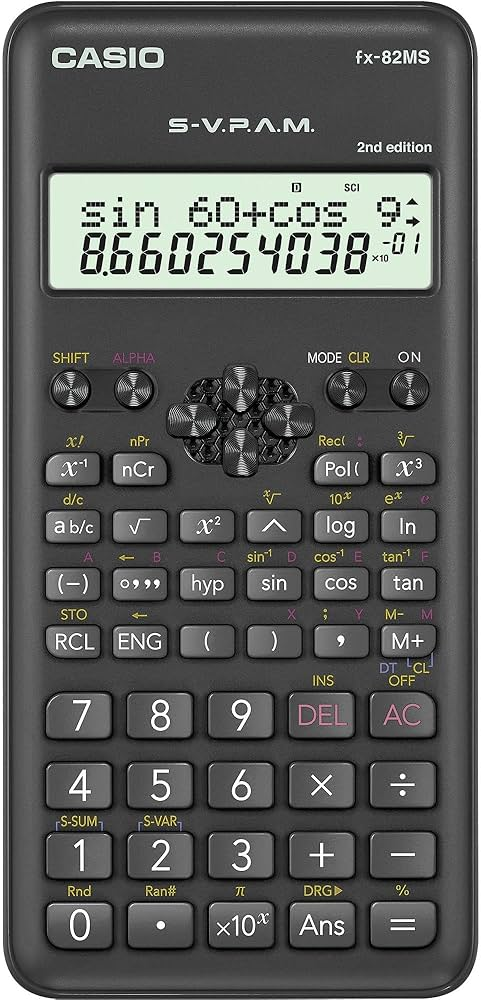
\includegraphics[width=0.58\textwidth]{img/casio-2ed.jpg}
        \caption{2\textsuperscript{a} Edição}
        \label{fig:ed2}
    \end{subfigure}
    \caption{Casio FX-82MS -- Edições}
\end{figure}

Apesar das alterações de projeto, as principais características funcionais da FX-82MS foram mantidas na segunda edição. Dessa forma, as diferenças apresentadas neste manual estão relacionadas principalmente à identificação visual e à disposição física dos elementos, e não à mudança do conteúdo estatístico abordado.

\subsection{Visor}

O visor da FX-82MS é composto por duas linhas: a linha superior exibe a 
expressão inserida pelo usuário, permitindo a conferência da entrada antes 
do cálculo, enquanto a linha inferior apresenta o resultado obtido. No topo 
do visor, pequenos indicadores informam o estado atual da calculadora:

\begin{itemize}
    \item \textbf{DEG / RAD / GRA} -- indica a unidade angular ativa para 
    cálculos trigonométricos;
    \item \textbf{M} -- indica que há um valor armazenado na memória 
    independente;
    \item \textbf{S} -- indica que a tecla \textbf{SHIFT} foi pressionada 
    e a próxima tecla ativará sua função secundária;
    \item \textbf{A} -- indica que a tecla \textbf{ALPHA} foi pressionada 
    e a próxima tecla ativará sua função terciária.
\end{itemize}

Esses indicadores são particularmente importantes durante a utilização dos recursos estatísticos e das funções acessadas por meio das teclas \textbf{SHIFT} e \textbf{ALPHA}, pois permitem identificar o estado atual da calculadora antes da execução de uma operação \cite{casio2004}.

\subsection{Teclado}

O teclado da FX-82MS é organizado de forma a concentrar múltiplas funções 
em cada tecla, reduzindo o tamanho físico do equipamento sem perda de 
funcionalidade. Cada tecla pode ter até três funções distintas:

\begin{itemize}
    \item \textbf{Função primária} -- indicada diretamente sobre a tecla, 
    ativada com um único pressionamento;
    \item \textbf{Função secundária} -- indicada em amarelo acima da tecla, 
    ativada pressionando \textbf{SHIFT} antes da tecla desejada;
    \item \textbf{Função terciária} -- indicada em vermelho acima da tecla, 
    ativada pressionando \textbf{ALPHA} antes da tecla desejada.
\end{itemize}

A identificação por cores permite localizar visualmente as funções disponíveis e compreender a sequência de teclas necessária para acessá-las \cite{casio2004}.

\subsection{Modos de Operação}

A FX-82MS oferece diferentes modos de operação, selecionados por meio da 
tecla \textbf{MODE}. A escolha do modo correto é fundamental para obter 
resultados esperados, pois cada modo altera o comportamento de diversas 
funções da calculadora:

\begin{itemize}
    \item \textbf{COMP (MODE 1)} -- modo de cálculo geral, utilizado para 
    operações aritméticas, trigonométricas, logarítmicas e demais cálculos 
    do dia a dia. É o modo padrão da calculadora;
    \item \textbf{SD (MODE 2)} -- modo de estatística com uma variável, 
    utilizado para cálculo de média, desvio padrão e soma de dados;
    \item \textbf{REG (MODE 3)} -- modo de regressão estatística, utilizado 
    para análise de correlação entre duas variáveis.
\end{itemize}

Para retornar ao modo padrão a qualquer momento, pressione \textbf{MODE}, 
em seguida \textbf{1}. Recomenda-se verificar o modo ativo antes de iniciar 
qualquer cálculo, especialmente após o uso das funções estatísticas.

\subsection{Ligando, Desligando e Reiniciando}

Para ligar a calculadora, pressione a tecla \textbf{ON}. Para desligá-la, pressione \textbf{SHIFT} seguido de \textbf{AC} (função \textbf{OFF}). A calculadora também possui um mecanismo de desligamento automático após um período sem utilização, contribuindo para a economia da bateria \cite{casio2004}.

O desligamento da calculadora não apaga os valores armazenados nas memórias. A Casio informa que a memória independente e os conteúdos das variáveis permanecem armazenados mesmo quando a calculadora é desligada \cite{casio2004}. Portanto, desligar e ligar novamente o equipamento não deve ser tratado como um procedimento de reinicialização das configurações.

Quando for necessário restaurar as configurações do modo de cálculo e de outras configurações, utilize a função \textbf{CLR}. O procedimento é:

\begin{itemize}
\item \textbf{SHIFT} $\rightarrow$ \textbf{CLR} $\rightarrow$ \textbf{2 (Mode)} -- restaura as configurações do modo de cálculo e da unidade angular para os valores iniciais;
\item \textbf{SHIFT} $\rightarrow$ \textbf{CLR} $\rightarrow$ \textbf{1 (Mcl)} -- limpa os conteúdos das memórias;
\item \textbf{SHIFT} $\rightarrow$ \textbf{CLR} $\rightarrow$ \textbf{3 (All)} -- restaura completamente a calculadora, apagando os dados armazenados e retornando as configurações aos valores iniciais.
\end{itemize}

A inicialização completa deve ser utilizada com cautela, pois remove os dados armazenados na memória da calculadora \cite{casio2004}.
\section{Operações Básicas}

A FX-82MS permite realizar as operações aritméticas fundamentais de forma direta, seguindo as regras de precedência matemática. O domínio dessas operações constitui uma etapa importante para a utilização posterior dos recursos estatísticos da calculadora, uma vez que muitos procedimentos envolvem a combinação de adições, subtrações, multiplicações, divisões e parênteses. Todos os exemplos desta seção assumem que a calculadora está no modo \textbf{COMP}, utilizado para cálculos gerais \cite{casio2004}.

\subsection{Operações Aritméticas}

As operações de adição, subtração, multiplicação e divisão são realizadas 
com as teclas \textbf{+}, \textbf{-}, \textbf{$\times$} e \textbf{$\div$}, 
respectivamente. A expressão é confirmada e calculada ao pressionar 
\textbf{=}.

Exemplo: calcular a média aritmética simples de três notas, operação 
fundamental em Probabilidade e Estatística. Dada a 
fórmula:

\begin{equation}
    \bar{x} = \frac{x_1 + x_2 + x_3}{n} = \frac{7 + 8 + 9}{3} = 8
\end{equation}

Na calculadora, a sequência de teclas é:

\begin{center}
\begin{tabular}{ll}
    \hline
    \textbf{Entrada} & \textbf{Resultado} \\
    \hline
    \texttt{( 7 + 8 + 9 ) / 3 =} & \texttt{8} \\
    \hline
\end{tabular}
\end{center}

\subsection{Números Negativos}

Números negativos são inseridos com a tecla \textbf{(-)}, localizada 
próxima à tecla \textbf{=}. Ela deve ser pressionada \emph{antes} do 
valor numérico, e não deve ser confundida com a tecla de subtração 
\textbf{-}, que opera entre dois operandos já existentes.

\begin{center}
\begin{tabular}{lll}
    \hline
    \textbf{Expressão} & \textbf{Entrada} & \textbf{Resultado} \\
    \hline
    $-5 + 3$ & \texttt{(-) 5 + 3 =} & \texttt{-2} \\
    $10 - (-4)$ & \texttt{10 - (-) 4 =}  & \texttt{14} \\
    $(-3) \times (-2)$ & \texttt{(-) 3 * (-) 2 =} & \texttt{6}  \\
    \hline
\end{tabular}
\end{center}

Utilizar a tecla \textbf{-} no lugar de \textbf{(-)} para introduzir um 
número negativo resultará em erro de sintaxe ou em cálculo incorreto, 
pois a calculadora interpretará o sinal como uma subtração sem operando 
à esquerda.

\subsection{Números Decimais}

A separação entre parte inteira e parte decimal é feita com a tecla 
\textbf{.} (ponto), independentemente da convenção regional de vírgula 
adotada no Brasil. Não há suporte para entrada com vírgula 
— seu uso causará erro de sintaxe.

\begin{center}
\begin{tabular}{lll}
    \hline
    \textbf{Expressão} & \textbf{Entrada} & \textbf{Resultado} \\
    \hline
    $1{,}5 + 2{,}3$ & \texttt{1.5 + 2.3 =} & \texttt{3.8} \\
    $7 \div 4$ & \texttt{7 / 4 =} & \texttt{1.75} \\
    $0{,}1 \times 0{,}2$ & \texttt{0.1 * 0.2 =} & \texttt{0.02} \\
    \hline
\end{tabular}
\end{center}

A FX-82MS exibe até dez dígitos significativos. Resultados com mais 
casas decimais são arredondados na exibição, mas o valor completo é 
mantido internamente e utilizado nos cálculos subsequentes via 
\textbf{Ans}, preservando a precisão \cite{casio2004}.

\subsection{Ordem de Operações e Parênteses}

A FX-82MS segue a ordem de precedência matemática padrão, conhecida 
pela hierarquia: potenciação, multiplicação e divisão, adição e subtração 
. Operações de mesma precedência são avaliadas da 
esquerda para a direita.

O uso de parênteses permite sobrescrever essa ordem, forçando a avaliação 
de uma subexpressão antes das demais. A calculadora suporta até 13 níveis 
de parênteses aninhados \cite{casio2004}.

Considere o exemplo abaixo, onde a ausência de parênteses altera 
completamente o resultado:

\begin{center}
\begin{tabular}{lll}
    \hline
    \textbf{Expressão} & \textbf{Entrada} & \textbf{Resultado} \\
    \hline
    $2 + 3 \times 4$ & \texttt{2 + 3 * 4 =} & \texttt{14} \\
    $(2 + 3) \times 4$ & \texttt{( 2 + 3 ) * 4 =} & \texttt{20} \\
    \hline
\end{tabular}
\end{center}

No primeiro caso, a multiplicação é resolvida antes da adição. No segundo, 
os parênteses forçam a adição primeiro. Recomenda-se sempre utilizar 
parênteses em expressões compostas, mesmo quando a precedência já 
garante o resultado correto, como boa prática de verificação.

\subsection{Correção de Entradas}

A FX-82MS oferece dois mecanismos de correção durante a digitação de uma 
expressão \cite{casio2004}:

\begin{itemize}
    \item \textbf{DEL} -- apaga o último caractere inserido na expressão, 
    permitindo corrigir erros pontuais sem reinserir toda a entrada. Pode 
    ser pressionada repetidamente para apagar vários caracteres;
    \item \textbf{AC} -- limpa completamente a expressão atual e o 
    resultado exibido no visor, reiniciando a entrada do zero. Não apaga 
    valores armazenados na memória independente \textbf{M} nem o conteúdo 
    da memória \textbf{Ans}.
\end{itemize}

Adicionalmente, as teclas de cursor \textbf{$\triangleleft$} e 
\textbf{$\triangleright$} permitem mover o cursor dentro da expressão 
digitada para corrigir um caractere em posição intermediária, sem apagar 
os demais.

\subsection{Reutilização do Resultado Anterior}

A memória \textbf{Ans} armazena automaticamente o resultado de cada 
cálculo realizado e pode ser recuperada pela tecla \textbf{Ans} 
\cite{casio2004}. Esse valor é atualizado a cada novo cálculo confirmado 
com \textbf{=} e persiste mesmo após pressionar \textbf{AC}.

O recurso é especialmente útil em cálculos encadeados, eliminando a 
necessidade de redigitar resultados intermediários e reduzindo a chance 
de erros de transcrição. Por exemplo, para calcular o desvio de cada nota 
em relação à média previamente obtida:

\begin{center}
\begin{tabular}{lll}
    \hline
    \textbf{Etapa} & \textbf{Entrada} & \textbf{Resultado} \\
    \hline
    Calcular a média & \texttt{( 7 + 8 + 9 ) / 3 =} & \texttt{8} \\
    Desvio da nota 9 & \texttt{9 - Ans =} & \texttt{1} \\
    Desvio da nota 7 & \texttt{7 - Ans =} & \texttt{-1} \\
    \hline
\end{tabular}
\end{center}

Importante: ao iniciar uma nova expressão pressionando diretamente 
\textbf{+}, \textbf{-}, \textbf{$\times$} ou \textbf{$\div$} logo após 
um resultado, a calculadora insere \textbf{Ans} automaticamente como 
primeiro operando, sem necessidade de pressionar a tecla explicitamente.

\subsection{Exemplos Práticos}

Esta subseção apresenta aplicações de operações aritméticas básicas com
exemplos contextualizados em Probabilidade e Estatística.

\subsubsection*{Exemplo 1 — Amplitude de um Conjunto de Dados}

A amplitude total é a diferença entre o maior e o menor valor de um
conjunto, e representa uma medida simples de dispersão. Dado o conjunto
de notas $\{4, 6, 7, 8, 9\}$:

\begin{equation}
    AT = x_{\max} - x_{\min} = 9 - 4 = 5
\end{equation}

\begin{center}
\begin{tabular}{lll}
    \hline
    \textbf{Expressão} & \textbf{Entrada} & \textbf{Resultado} \\
    \hline
    $x_{\max} - x_{\min}$ & \texttt{9 - 4 =} & \texttt{5} \\
    \hline
\end{tabular}
\end{center}

A amplitude indica que as notas variam em 5 pontos. Apesar de simples,
é frequentemente o primeiro passo antes de construir tabelas de
frequência.

\subsubsection*{Exemplo 2 — Média Ponderada}

Em avaliações com pesos distintos, a média ponderada é:

\begin{equation}
    \bar{x} = \frac{w_1 x_1 + w_2 x_2 + w_3 x_3}{w_1 + w_2 + w_3}
    = \frac{2 \cdot 6 + 3 \cdot 7 + 5 \cdot 9}{2 + 3 + 5}
\end{equation}

\begin{center}
\begin{tabular}{lll}
    \hline
    \textbf{Etapa} & \textbf{Entrada} & \textbf{Resultado} \\
    \hline
    Numerador & \texttt{( 2 * 6 + 3 * 7 + 5 * 9 ) =} & \texttt{78} \\
    Denominador & \texttt{Ans / ( 2 + 3 + 5 ) =} & \texttt{7.8} \\
    \hline
\end{tabular}
\end{center}

\subsubsection*{Exemplo 3 — Frequência relativa}

A frequência relativa expressa a proporção de cada valor em relação ao
total de observações, e é calculada dividindo a frequência absoluta pelo
total:

\begin{equation}
    fr_i = \frac{n_i}{n} \times 100
\end{equation}

Em uma turma de $30$ alunos, $12$ obtiveram nota entre $7{,}0$ e
$10{,}0$. A frequência relativa desse grupo é:

\begin{center}
\begin{tabular}{lll}
    \hline
    \textbf{Expressão} & \textbf{Entrada} & \textbf{Resultado} \\
    \hline
    $\dfrac{12}{30} \times 100$ & \texttt{12 / 30 * 100 =} & \texttt{40} \\
    \hline
\end{tabular}
\end{center}
\section{Potências e Raízes}

Potências e raízes são operações frequentes e aparecem em 
fórmulas de desvio padrão e variância. A FX-82MS oferece teclas dedicadas 
para as formas mais comuns dessas operações, e todas assumem que a 
calculadora está no modo \textbf{COMP} \cite{casio2004}.

\subsection{Quadrado e Cubo}

Para elevar um número ao quadrado, utilize a tecla \textbf{$x^2$}, 
localizada no painel central do teclado. Para elevar ao cubo, pressione 
\textbf{SHIFT} seguido de \textbf{$x^2$}, acessando a função secundária 
\textbf{$x^3$}. Ambas as funções são aplicadas ao valor imediatamente 
anterior ao cursor \cite{casio2004}.

Um exemplo de aplicação é o cálculo da variância amostral, que envolve elevar desvios ao quadrado:

\begin{equation}
    s^2 = \frac{(x_1 - \bar{x})^2 + (x_2 - \bar{x})^2 + (x_3 - \bar{x})^2}{n-1}
\end{equation}

\begin{center}
\begin{tabular}{lll}
    \hline
    \textbf{Expressão} & \textbf{Entrada} & \textbf{Resultado} \\
    \hline
    $5^2$ & \texttt{5 $x^2$ =} & \texttt{25} \\
    $3^3$ & \texttt{3 SHIFT $x^2$ =} & \texttt{27} \\
    \hline
\end{tabular}
\end{center}

\subsection{Potência de Expoente Qualquer}

Para calcular uma potência com expoente arbitrário, utilize a tecla
\textbf{$\wedge$}. A sintaxe é: digite a base, pressione a tecla, digite
o expoente e confirme com \textbf{=} \cite{casio2004}.

\begin{center}
\begin{tabular}{lll}
    \hline
    \textbf{Expressão} & \textbf{Entrada} & \textbf{Resultado} \\
    \hline
    $2^{10}$ & \texttt{2 \^{} 10 =} & \texttt{1024} \\
    $3^4$ & \texttt{3 \^{} 4 =} & \texttt{81} \\
    $(-2)^3$ & \texttt{( (-) 2 ) \^{} 3 =} & \texttt{-8} \\
    \hline
\end{tabular}
\end{center}

Atenção: ao calcular potências de bases negativas, utilize parênteses ao
redor da base para garantir que o sinal negativo seja incluído
corretamente na operação. Sem os parênteses, a calculadora pode
interpretar a expressão de forma distinta do esperado \cite{casio2004}.

\subsection{Raiz Quadrada e Cúbica}

A raiz quadrada é acessada diretamente pela tecla 
\textbf{$\sqrt{\phantom{x}}$}, que precede o radicando. A raiz cúbica é 
acessada via \textbf{SHIFT} seguido da tecla de raiz quadrada, ativando 
a função \textbf{$\sqrt[3]{\phantom{x}}$} \cite{casio2004}.

O desvio padrão amostral envolve o cálculo de uma raiz quadrada:

\begin{equation}
    s = \sqrt{\frac{\sum_{i=1}^{n}(x_i - \bar{x})^2}{n-1}}
\end{equation}

\begin{center}
\begin{tabular}{lll}
    \hline
    \textbf{Expressão} & \textbf{Entrada} & \textbf{Resultado} \\
    \hline
    $\sqrt{144}$ & \texttt{$\sqrt{\phantom{x}}$ 144 =} & \texttt{12} \\
    $\sqrt{2}$ & \texttt{$\sqrt{\phantom{x}}$ 2 =} & \texttt{1.414213562} \\
    $\sqrt[3]{27}$ & \texttt{SHIFT $\sqrt{\phantom{x}}$ 27 =} & \texttt{3} \\
    \hline
\end{tabular}
\end{center}

\subsection{Raiz de Índice Qualquer}

Para raízes de índice arbitrário, utilize a função \textbf{$x^{1/y}$}, 
acessada via \textbf{SHIFT} seguido da tecla \textbf{$\wedge$}. A sintaxe 
é: digite o índice da raiz, pressione \textbf{SHIFT} e a tecla, depois 
digite o radicando e confirme com \textbf{=} \cite{casio2004}.

\begin{equation}
    \sqrt[y]{x} = x^{1/y}
\end{equation}

\begin{center}
\begin{tabular}{lll}
    \hline
    \textbf{Expressão} & \textbf{Entrada} & \textbf{Resultado} \\
    \hline
    $\sqrt[4]{625}$ & \texttt{4 SHIFT \^{} 625 =} & \texttt{5} \\
    $\sqrt[5]{32}$ & \texttt{5 SHIFT \^{} 32 =} & \texttt{2} \\
    \hline
\end{tabular}
\end{center}

Ressalta-se que raízes de índice par aplicadas a radicandos negativos 
resultam em erro no domínio real (\texttt{Math ERROR}), pois a FX-82MS 
não opera com números complexos \cite{casio2004}.

\subsection{Combinação Simples}

O cálculo de combinações simples é utilizado na determinação do número de agrupamentos não ordenados de $k$ elementos escolhidos a partir de um total de $n$ elementos. A FX-82MS dispõe da tecla dedicada \textbf{nCr} para realizar esse cálculo diretamente, sem a necessidade de expandir os fatoriais da fórmula \cite{casio2004}:

\begin{equation}
    \binom{n}{k} = C_{n,k} = \frac{n!}{k!(n-k)!}
\end{equation}

A sintaxe de entrada na calculadora é: digite o valor total de elementos ($n$), pressione a tecla \textbf{nCr}, digite a quantidade de elementos agrupados ($k$) e confirme com \textbf{=} \cite{casio2004}.

\begin{center}
\begin{tabular}{lll}
    \hline
    \textbf{Expressão} & \textbf{Entrada} & \textbf{Resultado} \\
    \hline
    $\binom{5}{2}$ & \texttt{5 nCr 2 =} & \texttt{10} \\
    $\binom{10}{3}$ & \texttt{10 nCr 3 =} & \texttt{120} \\
    \hline
\end{tabular}
\end{center}

Essa função constitui o elemento central para a resolução de problemas baseados na \textbf{Distribuição Binomial} no modo \textbf{COMP}, na qual a probabilidade de obter $k$ sucessos em $n$ ensaios independentes é dada por:

\begin{equation}
    P(X = k) = \binom{n}{k} \cdot p^k \cdot (1-p)^{n-k}
\end{equation}

\subsection{Números Negativos e Domínio das Operações}

A FX-82MS opera exclusivamente no domínio dos números reais, o que impõe
restrições a certas combinações de base, expoente e radicando
\cite{casio2004}. Quando uma operação resulta em valor fora desse domínio,
a calculadora exibe \texttt{Math ERROR} e interrompe o cálculo.

As situações mais comuns que produzem esse erro são \cite{casio2004}:

\begin{itemize}
    \item \textbf{Raiz de índice par com radicando negativo} -- por exemplo,
    $\sqrt{-4}$ ou $\sqrt[4]{-16}$, cujos resultados são imaginários;
    \item \textbf{Potência de base negativa com expoente fracionário} --
    por exemplo, $(-8)^{0{,}5}$, equivalente a $\sqrt{-8}$ no reais;
    \item \textbf{Raiz de índice par com expoente fracionário não simplificável}
    -- casos em que a calculadora não consegue determinar um resultado real.
\end{itemize}

Raízes de índice \emph{ímpar} aplicadas a radicandos negativos, por outro
lado, são válidas no domínio real e calculadas corretamente:

\begin{center}
\begin{tabular}{lll}
    \hline
    \textbf{Expressão} & \textbf{Entrada} & \textbf{Resultado} \\
    \hline
    $\sqrt[3]{-8}$  & \texttt{SHIFT $\sqrt{\phantom{x}}$ (-) 8 =} & \texttt{-2} \\
    $(-2)^3$ & \texttt{( (-) 2 ) \^{} 3 =} & \texttt{-8} \\
    $(-2)^4$ & \texttt{( (-) 2 ) \^{} 4 =} & \texttt{16} \\
    $\sqrt{-4}$ & \texttt{$\sqrt{\phantom{x}}$ (-) 4 =} & \texttt{Math ERROR} \\
    \hline
\end{tabular}
\end{center}

Ao encontrar \texttt{Math ERROR}, pressione \textbf{AC} para limpar o
visor e revisar a expressão antes de recalcular.

\subsection{Exemplos Práticos}

Esta subseção apresenta aplicações de potências e raízes com
exemplos contextualizados em Probabilidade e Estatística.

\subsubsection*{Exemplo 1 — Desvio padrão amostral}

Dadas as notas $6$, $8$ e $10$, com média $\bar{x} = 8$, o desvio padrão
amostral é:

\begin{equation}
    s = \sqrt{\frac{(6-8)^2 + (8-8)^2 + (10-8)^2}{3-1}}
      = \sqrt{\frac{4 + 0 + 4}{2}} = \sqrt{4} = 2
\end{equation}

O cálculo é realizado em etapas, aproveitando a memória \textbf{Ans}
para encadear os resultados intermediários:

\begin{center}
\begin{tabular}{lll}
    \hline
    \textbf{Etapa} & \textbf{Entrada} & \textbf{Resultado} \\
    \hline
    Soma dos quadrados & \texttt{( 6 - 8 ) $x^2$ + ( 8 - 8 ) $x^2$ + ( 10 - 8 ) $x^2$ =} & \texttt{8} \\
    Variância amostral & \texttt{Ans / ( 3 - 1 ) =} & \texttt{4} \\
    Desvio padrão & \texttt{$\sqrt{\phantom{x}}$ Ans =} & \texttt{2} \\
    \hline
\end{tabular}
\end{center}

\subsubsection*{Exemplo 2 — Variância populacional}

Uma pesquisa registrou os seguintes tempos de atendimento em minutos:
$2$, $4$, $4$, $4$, $5$, $5$, $7$ e $9$. A média é $\bar{x} = 5$ e
a variância populacional é:

\begin{equation}
    s^2 = \frac{\sum_{i=1}^{n}(x_i - \bar{x})^2}{n}
             = \frac{9 + 1 + 1 + 1 + 0 + 0 + 4 + 16}{8}
             = \frac{32}{8} = 4
\end{equation}

\begin{center}
\begin{tabular}{lll}
    \hline
    \textbf{Etapa} & \textbf{Entrada} & \textbf{Resultado} \\
    \hline
    Soma dos quadrados & \texttt{( 2 - 5 ) $x^2$ + ( 4 - 5 ) $x^2$ +} & \\
                       & \texttt{( 4 - 5 ) $x^2$ + ( 4 - 5 ) $x^2$ +} & \\
                       & \texttt{( 5 - 5 ) $x^2$ + ( 5 - 5 ) $x^2$ +} & \\
                       & \texttt{( 7 - 5 ) $x^2$ + ( 9 - 5 ) $x^2$ =} & \texttt{32} \\
    Variância & \texttt{Ans / 8 =} & \texttt{4} \\
    Desvio padrão & \texttt{$\sqrt{\phantom{x}}$ Ans =} & \texttt{2} \\
    \hline
\end{tabular}
\end{center}

\subsubsection*{Exemplo 3 — Coeficiente de variação}

O coeficiente de variação ($CV$) expressa o desvio padrão como percentual
da média, permitindo comparar a dispersão de conjuntos com unidades ou
magnitudes diferentes:

\begin{equation}
    CV = \frac{s}{\bar{x}} \times 100
\end{equation}

Considere duas turmas com os seguintes resultados em uma avaliação:

\begin{itemize}
    \item Turma A: $\bar{x} = 8{,}0$ e $s = 2{,}0$
    \item Turma B: $\bar{x} = 6{,}0$ e $s = 1{,}8$
\end{itemize}

\begin{center}
\begin{tabular}{lll}
    \hline
    \textbf{Etapa} & \textbf{Entrada} & \textbf{Resultado} \\
    \hline
    $CV$ Turma A & \texttt{2 / 8 * 100 =}   & \texttt{25} \\
    $CV$ Turma B & \texttt{1.8 / 6 * 100 =} & \texttt{30} \\
    \hline
\end{tabular}
\end{center}

\section{Memória e Armazenamento de Valores}

A FX-82MS dispõe de recursos de memória que permitem armazenar e recuperar
valores intermediários durante a realização de cálculos. O uso adequado desses
recursos evita a necessidade de redigitar resultados obtidos em etapas anteriores,
reduzindo a possibilidade de erros de transcrição e tornando o processo de cálculo
mais eficiente. A calculadora oferece dois tipos principais de armazenamento: a
memória independente e as variáveis de A a F, M, X e Y \cite{casio2004}.

\subsection{Memória Independente}

A memória independente, identificada pela letra \textbf{M} no visor, permite
acumular valores ao longo de uma sequência de cálculos. Ela é gerenciada por
meio de três operações principais \cite{casio2004}:

\begin{itemize}
    \item \textbf{M+} -- adiciona o resultado atual ao valor armazenado em M;
    \item \textbf{SHIFT} seguido de \textbf{M+} (função \textbf{M$-$}) -- subtrai o resultado atual do valor armazenado em M;
    \item \textbf{RCL} seguido de \textbf{M+} -- recupera o valor armazenado em M e o exibe no visor.
\end{itemize}

O indicador \textbf{M} aparece no topo do visor sempre que há um valor diferente
de zero armazenado na memória independente. Para zerar a memória M sem apagar
as demais configurações, armazene o valor zero com a sequência
\textbf{0} $\to$ \textbf{M+}, ou utilize \textbf{SHIFT} $\to$ \textbf{CLR} $\to$
\textbf{1} (Mcl), que limpa todas as memórias simultaneamente
\cite{casio2004}.

Uma aplicação direta da memória independente é o cálculo de somas acumuladas,
como a soma dos quadrados dos desvios utilizada no cálculo da variância. Dadas as
notas 6, 7 e 8, com média $\bar{x} = 7$:

\begin{table}[H]
    \centering
    \begin{tabular}{lll}
        \hline
        \textbf{Etapa} & \textbf{Entrada} & \textbf{Resultado} \\ \hline
            Zerar a memória & \texttt{0 M+} & M = 0 \\
            Primeiro quadrado & \texttt{( 6 - 7 ) x\textasciicircum{}2 M+} & M = 1 \\
            Segundo quadrado & \texttt{( 7 - 7 ) x\textasciicircum{}2 M+} & M = 1 \\
            Terceiro quadrado & \texttt{( 8 - 7 ) x\textasciicircum{}2 M+} & M = 2 \\
            Recuperar o total & \texttt{RCL M+} & 2 \\
            Variância amostral & \texttt{Ans / ( 3 - 1 ) =} & 1 \\ \hline
        \end{tabular}
\end{table}

O valor acumulado em M permanece armazenado mesmo após pressionar \textbf{AC}
ou desligar a calculadora, o que exige atenção: recomenda-se sempre zerar a
memória independente antes de iniciar um novo cálculo que faça uso de M+,
evitando que valores residuais de operações anteriores interfiram no resultado.

\subsection{Variáveis de Armazenamento}

Além da memória independente, a FX-82MS disponibiliza oito variáveis de
armazenamento identificadas pelas letras \textbf{A}, \textbf{B}, \textbf{C},
\textbf{D}, \textbf{E}, \textbf{F}, \textbf{X} e \textbf{Y}, além da variável
\textbf{M}, compartilhada com a memória independente, totalizando nove variáveis
disponíveis \cite{casio2004}. Cada variável armazena um único valor
numérico e pode ser acessada individualmente, o que as torna adequadas para
guardar constantes ou resultados intermediários que serão reutilizados em
diferentes etapas de um mesmo cálculo \cite{casio2004}.

O armazenamento de um valor em uma variável é feito com a tecla \textbf{STO},
seguida da tecla correspondente à variável desejada. A recuperação do valor
armazenado é feita com a tecla \textbf{RCL}, também seguida da tecla da variável.
As letras A a F e M estão indicadas em vermelho acima de teclas específicas e são
acessadas por meio da tecla \textbf{ALPHA} \cite{casio2004}:

\begin{itemize}
    \item \textbf{STO} $\to$ \textbf{ALPHA} $\to$ \textit{tecla da variável} -- armazena o valor atual na variável indicada;
    \item \textbf{RCL} $\to$ \textbf{ALPHA} $\to$ \textit{tecla da variável} -- recupera o valor armazenado na variável indicada.
\end{itemize}

O conteúdo de cada variável permanece armazenado após pressionar \textbf{AC}
ou desligar a calculadora. Para limpar todas as variáveis simultaneamente,
utilize \textbf{SHIFT} $\to$ \textbf{CLR} $\to$ \textbf{1} (Mcl). A
reinicialização completa por meio de \textbf{SHIFT} $\to$ \textbf{CLR} $\to$
\textbf{3} (All) também apaga o conteúdo de todas as variáveis
\cite{casio2004}.

Um uso típico das variáveis é o armazenamento da média de um conjunto de dados
para reutilização no cálculo dos desvios individuais, evitando redigitar o valor
a cada etapa. Considere as notas 5, 7 e 9, cuja média é $\bar{x} = 7$:

\begin{table}[H]
    \centering
        \begin{tabular}{lll}
        \hline
        \textbf{Etapa} & \textbf{Entrada} & \textbf{Resultado} \\ \hline
            Calcular a média & \texttt{( 5 + 7 + 9 ) / 3 =} & 7 \\
            Armazenar em A & \texttt{STO ALPHA A} & 7 \\
            Desvio da nota 5 & \texttt{5 - RCL ALPHA A =} & -2 \\
            Desvio da nota 7 & \texttt{7 - RCL ALPHA A =} & 0 \\
            Desvio da nota 9 & \texttt{9 - RCL ALPHA A =} & 2 \\ \hline
        \end{tabular}
\end{table}

É importante distinguir o papel da variável \textbf{M} do papel da memória
independente, embora compartilhem o mesmo espaço de armazenamento: ao utilizar
\textbf{M+} ou \textbf{M$-$}, o valor em M é acumulado; ao utilizar
\textbf{STO} $\to$ \textbf{M}, o valor atual \emph{substitui} o conteúdo
anterior de M, sem acumulação. Essa distinção é relevante para evitar
comportamentos inesperados quando as duas formas de acesso à memória M são
combinadas em um mesmo cálculo \cite{casio2004}.

\subsection{Uso Estratégico em Cálculos Estatísticos}

A combinação entre a memória independente e as variáveis de armazenamento
permite estruturar cálculos estatísticos de forma organizada e sem retrabalho.
Uma estratégia eficiente consiste em armazenar valores fixos, como a média ou
um denominador comum, nas variáveis A a F, enquanto a memória M acumula
somas parciais ao longo das etapas \cite{casio2004}.

Essa abordagem é especialmente útil no cálculo da variância e do desvio padrão,
em que o mesmo valor da média é subtraído repetidamente de cada dado do
conjunto. Ao armazenar a média em uma variável antes de iniciar os cálculos dos
desvios, evita-se a redigitação do valor a cada etapa, reduzindo o risco de erro.

Ao final de uma sequência de cálculos que envolva M+, recomenda-se recuperar
o valor acumulado com \textbf{RCL M+} antes de prosseguir com as operações
seguintes. Quando o mesmo cálculo envolver tanto \textbf{STO M} quanto
\textbf{M+}, é importante ter clareza sobre qual operação está sendo utilizada
em cada etapa, uma vez que o comportamento de acumulação e de substituição
diferem, conforme descrito na seção anterior.

\subsection{Exemplos Práticos}

Os exemplos a seguir combinam o uso das variáveis de armazenamento e da
memória independente para resolver problemas completos.

\subsubsection*{Exemplo 1 -- Desvio padrão amostral}

Dado o conjunto de valores \{4, 7, 7, 10\}, calcule o desvio padrão amostral $s$. A média é $\bar{x} = (4 + 7 + 7 + 10)/4 = 7$. Armazena-se a média na variável A e acumulam-se os quadrados dos desvios na memória M:

\begin{table}[H]
    \centering
    \begin{tabular}{lll}
        \hline
        \textbf{Etapa} & \textbf{Entrada} & \textbf{Resultado} \\ \hline
            Calcular a média & \texttt{( 4 + 7 + 7 + 10 ) / 4 =} & 7 \\
            Armazenar em A & \texttt{STO ALPHA A} & 7 \\
            Zerar memória M & \texttt{0 M+} & M = 0 \\
            Desvio de 4 & \texttt{( 4 - RCL ALPHA A ) x\textasciicircum{}2 M+} & M = 9 \\
            Desvio de 7 (1º) & \texttt{( 7 - RCL ALPHA A ) x\textasciicircum{}2 M+} & M = 9 \\
            Desvio de 7 (2º) & \texttt{( 7 - RCL ALPHA A ) x\textasciicircum{}2 M+} & M = 9 \\
            Desvio de 10 & \texttt{( 10 - RCL ALPHA A ) x\textasciicircum{}2 M+} & M = 18 \\
            Recuperar soma & \texttt{RCL M+} & 18 \\
            Variância amostral & \texttt{Ans / ( 4 - 1 ) =} & 6 \\
            Desvio padrão & \texttt{$\sqrt{\phantom{0}}$ Ans =} & $\approx 2{,}449$ \\ \hline
    \end{tabular}
\end{table}

\subsubsection*{Exemplo 2 -- Média ponderada} 

Um aluno obteve as notas 6,0, 8,0 e 5,0 nas provas P1, P2 e P3, com pesos 2, 3 e 5, respectivamente. Calcule a média ponderada $\bar{x}$.

Armazena-se o denominador (soma dos pesos) na variável B e acumula-se o numerador (soma dos produtos nota $\times$ peso) na memória M:

\begin{table}[H]
    \centering
    \begin{tabular}{lll}
        \hline
        \textbf{Etapa} & \textbf{Entrada} & \textbf{Resultado} \\ \hline
            Armazenar soma dos pesos & \texttt{( 2 + 3 + 5 ) = STO ALPHA B} & 10 \\
            Zerar memória M & \texttt{0 M+} & M = 0 \\
            Produto P1 & \texttt{6 $\times$ 2 M+} & M = 12 \\
            Produto P2 & \texttt{8 $\times$ 3 M+} & M = 36 \\
            Produto P3 & \texttt{5 $\times$ 5 M+} & M = 61 \\
            Recuperar numerador & \texttt{RCL M+} & 61 \\
            Média ponderada & \texttt{Ans / RCL ALPHA B =} & 6{,}1 \\ \hline
    \end{tabular}
\end{table}
\section{Cálculos Estatísticos}

A FX-82MS dispõe de um modo dedicado a cálculos estatísticos com uma
variável, denominado Modo SD (\textit{Standard Deviation}). Nesse modo, a
calculadora mantém um editor interno de dados e disponibiliza funções para
o cálculo automático de média, desvio padrão e outras grandezas derivadas,
eliminando a necessidade de realizar essas operações manualmente etapa por
etapa \cite{casio2004}.

Para ativar o Modo SD, pressione \textbf{MODE} seguido de \textbf{2}. O
visor exibirá o indicador \textbf{SD} no topo, confirmando que a calculadora
está pronta para receber dados estatísticos \cite{casio2004}. Recomenda-se
limpar os dados de sessões anteriores antes de iniciar uma nova entrada,
utilizando a sequência \textbf{SHIFT} $\to$ \textbf{CLR} $\to$ \textbf{1}
(Scl), que apaga todos os dados do editor sem alterar as demais configurações
da calculadora.

\subsection{Inserindo e Editando Dados}

No Modo SD, os dados são inseridos um a um por meio da tecla \textbf{DT},
que corresponde à função secundária da tecla \textbf{M+}. Cada valor deve
ser digitado e confirmado com \textbf{DT}; o visor exibe brevemente o número
de elementos inseridos até o momento, identificado no visor como \textbf{n}
\cite{casio2004}.

Para inserir os valores 4, 7 e 9, por exemplo, a sequência é:

\begin{table}[H]
    \centering
    \begin{tabular}{lll}
        \hline
        \textbf{Etapa} & \textbf{Entrada} & \textbf{Visor} \\ \hline
        Ativar Modo SD & \texttt{MODE 2} & SD \\
        Limpar dados & \texttt{SHIFT CLR 1} & 0 \\
        Inserir primeiro valor & \texttt{4 DT} & n = 1 \\
        Inserir segundo valor & \texttt{7 DT} & n = 2 \\
        Inserir terceiro valor & \texttt{9 DT} & n = 3 \\ \hline
    \end{tabular}
\end{table}

Caso um valor tenha sido inserido incorretamente, é possível removê-lo
sem apagar todo o conjunto. Para excluir uma entrada, redigite o valor
incorreto e pressione \textbf{SHIFT} seguido de \textbf{DT} (função
\textbf{CD} -- \textit{Count Down}), que remove a última ocorrência daquele
valor do editor \cite{casio2004}. Em seguida, insira o valor correto
normalmente com \textbf{DT}.

É importante observar que a FX-82MS não permite visualizar ou navegar
pela lista de dados inseridos. Por isso, recomenda-se anotar os valores em
papel à medida que são inseridos, facilitando a identificação e correção de
eventuais erros.

\subsection{Média e Soma}

Após a inserção dos dados no Modo SD, a FX-82MS disponibiliza as
grandezas estatísticas por meio da tecla \textbf{SHIFT} seguida de
\textbf{2} (função \textbf{S-VAR}), que abre um menu com as variáveis
estatísticas disponíveis \cite{casio2004}. A média aritmética e as somas
acumuladas são acessadas por esse menu e exibidas no visor ao confirmar
com \textbf{=}.

As grandezas relacionadas à média e à soma são \cite{casio2004}:

\begin{itemize}
    \item $\bar{x}$ \textbf{(S-VAR 1)} -- média aritmética dos valores inseridos,
    calculada automaticamente pela calculadora como:
    \begin{equation}
        \bar{x} = \frac{\sum x_i}{n}
    \end{equation}
    \item $\sum x$ \textbf{(S-VAR 4)} -- soma de todos os valores inseridos;
    \item $\sum x^2$ \textbf{(S-VAR 5)} -- soma dos quadrados de todos os valores inseridos;
    \item $n$ \textbf{(S-VAR 6)} -- número total de elementos inseridos.
\end{itemize}

Para recuperar qualquer uma dessas grandezas, pressione \textbf{SHIFT}
$\to$ \textbf{2} (S-VAR), selecione o número correspondente à grandeza
desejada e confirme com \textbf{=}. Considerando o conjunto \{4, 7, 9\}
já inserido:

\begin{table}[H]
    \centering
    \begin{tabular}{lll}
        \hline
        \textbf{Grandeza} & \textbf{Entrada} & \textbf{Resultado} \\ \hline
        Média $\bar{x}$ & \texttt{SHIFT 2 1 =} & 6{,}666\ldots \\
        Soma $\sum x$ & \texttt{SHIFT 2 4 =} & 20 \\
        Soma $\sum x^2$ & \texttt{SHIFT 2 5 =} & 146 \\
        Total $n$ & \texttt{SHIFT 2 6 =} & 3 \\ \hline
    \end{tabular}
\end{table}

O valor de $\bar{x}$ retornado pela calculadora é mantido internamente
com precisão completa, mesmo que o visor exiba uma versão arredondada.
Ao utilizar o resultado de $\bar{x}$ em cálculos subsequentes por meio
da tecla \textbf{Ans}, a precisão total é preservada, evitando erros de
arredondamento acumulado \cite{casio2004}.

\subsection{Desvio Padrão}

O desvio padrão é uma medida de dispersão que indica o quanto os valores
de um conjunto se afastam, em média, da média aritmética. A FX-82MS calcula
automaticamente duas versões do desvio padrão no Modo SD, acessíveis pelo
mesmo menu \textbf{S-VAR} utilizado para a média e as somas
\cite{casio2004}.

A distinção entre as duas versões está na natureza do conjunto de dados
analisado: se os dados representam a população completa, utiliza-se o desvio
padrão populacional; se representam uma amostra extraída de uma população
maior, utiliza-se o desvio padrão amostral \cite{casio2004}.

\subsubsection{Desvio Padrão Populacional}

O desvio padrão populacional $s x$ considera que os dados inseridos
representam todos os elementos da população. Sua fórmula é \cite{casio2004}:

\begin{equation}
    s_1 = \sqrt{\frac{\sum (x_i - \bar{x})^2}{n}}
\end{equation}

É acessado por meio de \textbf{SHIFT} $\to$ \textbf{2} (S-VAR) $\to$
\textbf{2}. Considerando o conjunto \{4, 7, 9\}:

\begin{table}[H]
    \centering
    \begin{tabular}{lll}
        \hline
        \textbf{Grandeza} & \textbf{Entrada} & \textbf{Resultado} \\ \hline
        Desvio padrão populacional $s_1$ & \texttt{SHIFT 2 2 =} & $\approx 2{,}055$ \\ \hline
    \end{tabular}
\end{table}

\subsubsection{Desvio Padrão Amostral}

O desvio padrão amostral $s_2$ considera que os dados inseridos representam
uma amostra da população, aplicando a correção de Bessel no denominador para
produzir uma estimativa não tendenciosa \cite{casio2004}:

\begin{equation}
    s_2 = \sqrt{\frac{\sum (x_i - \bar{x})^2}{n - 1}}
\end{equation}

É acessado por meio de \textbf{SHIFT} $\to$ \textbf{2} (S-VAR) $\to$
\textbf{3}. Para o mesmo conjunto \{4, 7, 9\}:

\begin{table}[H]
    \centering
    \begin{tabular}{lll}
        \hline
        \textbf{Grandeza} & \textbf{Entrada} & \textbf{Resultado} \\ \hline
        Desvio padrão amostral $s_2$ & \texttt{SHIFT 2 3 =} & $\approx 2{,}517$ \\ \hline
    \end{tabular}
\end{table}

A diferença entre $s_1$ e $s_2$ é mais pronunciada em conjuntos
pequenos e tende a diminuir à medida que $n$ cresce. Em contextos acadêmicos,
o enunciado do problema geralmente indica qual versão utilizar; na ausência
dessa informação, recomenda-se verificar se os dados representam uma
população completa ou uma amostra antes de escolher a função adequada.

\subsection{Outras Grandezas Disponíveis}

Além da média e dos desvios padrão apresentados nas seções anteriores, o
menu S-VAR reúne todas as grandezas calculadas automaticamente pela
calculadora a partir dos dados inseridos no Modo SD. A tabela a seguir
apresenta uma visão consolidada das seis grandezas disponíveis, com os
respectivos atalhos e significados \cite{casio2004}.

\begin{table}[H]
    \centering
    \begin{tabular}{lll}
        \hline
        \textbf{Atalho} & \textbf{Grandeza} & \textbf{Significado} \\ \hline
        \texttt{SHIFT 2 1} & $\bar{x}$    & Média aritmética \\
        \texttt{SHIFT 2 2} & $s_1$        & Desvio padrão populacional \\
        \texttt{SHIFT 2 3} & $s_2$        & Desvio padrão amostral \\
        \texttt{SHIFT 2 4} & $\sum x$     & Soma dos valores \\
        \texttt{SHIFT 2 5} & $\sum x^2$   & Soma dos quadrados dos valores \\
        \texttt{SHIFT 2 6} & $n$          & Número de elementos \\ \hline
    \end{tabular}
\end{table}

Os resultados do menu S-VAR podem ser utilizados diretamente em cálculos
subsequentes por meio da tecla \textbf{Ans} \cite{casio2004}, permitindo
derivar grandezas que não constam no menu, como a variância e o coeficiente
de variação. A variância corresponde ao quadrado do desvio padrão e pode ser
obtida elevando o resultado retornado pelo menu ao quadrado com a tecla $x^2$:

\begin{table}[H]
    \centering
    \begin{tabular}{lll}
        \hline
        \textbf{Etapa} & \textbf{Entrada} & \textbf{Resultado} \\ \hline
        Recuperar $s_2$ & \texttt{SHIFT 2 3 =}  & valor de $s_2$ \\
        Variância amostral $s_2^2$ & \texttt{Ans x\textsuperscript{2} =} & $s_2^2$ \\ \hline
    \end{tabular}
\end{table}

Para o conjunto \{4, 7, 9\} utilizado nas seções anteriores, o valor
$s_2 \approx 2{,}517$ resulta em variância amostral $s_2^2 \approx 6{,}333$.
De modo análogo, a variância populacional obtida a partir de $s_1 \approx 2{,}055$
é $s_1^2 \approx 4{,}222$.

\subsection{Dados com Frequência}

Quando os dados provêm de uma tabela de frequências ou contêm valores
repetidos, a FX-82MS permite inserir cada valor acompanhado de sua frequência
absoluta, evitando a digitação individual de cada ocorrência. Esse recurso é
especialmente útil em exercícios de Estatística que apresentam os dados já
resumidos em tabelas \cite{casio2004}.

No Modo SD, a entrada de um valor $x$ com frequência $f$ é realizada pela
sequência \cite{casio2004}:

\begin{center}
    \textit{valor} \textbf{;} \textit{frequência} \textbf{DT}
\end{center}

Onde o separador \textbf{;} é acessado pela tecla correspondente do teclado,
conforme indicado no painel da calculadora. Ao confirmar com \textbf{DT}, o
visor exibe o número total acumulado de elementos $n$, já computando a
frequência informada. Quando a frequência é igual a 1, o separador pode ser
omitido e o valor inserido diretamente com \textbf{DT}.

Considere o conjunto de tempos de atendimento \{2, 4, 4, 4, 5, 5, 7, 9\}, cujos valores repetidos tornam a
entrada por frequência vantajosa. Sua tabela de frequências é:

\begin{table}[H]
    \centering
    \begin{tabular}{ll}
        \hline
        \textbf{Valor} ($x_i$) & \textbf{Frequência} ($f_i$) \\ \hline
        2 & 1 \\
        4 & 3 \\
        5 & 2 \\
        7 & 1 \\
        9 & 1 \\ \hline
    \end{tabular}
\end{table}

A inserção com frequência reduz o número de entradas de 8 para 5:

\begin{table}[htbp]
    \centering
    \begin{tabular}{lll}
        \hline
        \textbf{Etapa} & \textbf{Entrada} & \textbf{Visor} \\ \hline
        Ativar Modo SD      & \texttt{MODE 2}       & SD    \\
        Limpar dados        & \texttt{SHIFT CLR 1}  & 0     \\
        Valor 2, freq.\ 1  & \texttt{2 DT}         & n = 1 \\
        Valor 4, freq.\ 3  & \texttt{4 ; 3 DT}     & n = 4 \\
        Valor 5, freq.\ 2  & \texttt{5 ; 2 DT}     & n = 6 \\
        Valor 7, freq.\ 1  & \texttt{7 DT}         & n = 7 \\
        Valor 9, freq.\ 1  & \texttt{9 DT}         & n = 8 \\ \hline
    \end{tabular}
\end{table}

Após a inserção, as grandezas estatísticas são recuperadas normalmente pelo
menu S-VAR, com $n = 8$ elementos computados de acordo com as frequências
informadas. O conjunto inserido por frequência é equivalente, para fins de
cálculo, à inserção individual de todos os elementos \cite{casio2004}.

Para remover uma entrada inserida com frequência incorreta, redigite o valor
e a frequência no mesmo formato e pressione \textbf{SHIFT} seguido de
\textbf{DT} (função \textbf{CD}).

\subsection{Exemplos Práticos}

Esta subseção apresenta aplicações de cálculos estatísticos com
exemplos contextualizados em Probabilidade e Estatística.

\subsubsection*{Exemplo 1 — Distribuição Binomial}

Em um processo de fabricação, a probabilidade de uma peça apresentar defeito é $p = 0{,}2$ ($20\%$). Se $5$ peças forem selecionadas aleatoriamente, calcule a probabilidade de exatamente $2$ peças serem defeituosas ($k = 2$).

A probabilidade em uma Distribuição Binomial é calculada pela fórmula:

\begin{equation}
    P(X = k) = \binom{n}{k} \cdot p^k \cdot (1-p)^{n-k}
\end{equation}

Para $n = 5$, $k = 2$, $p = 0{,}2$ e $(1-p) = 0{,}8$:

\begin{equation}
    P(X = 2) = \binom{5}{2} \cdot (0{,}2)^2 \cdot (0{,}8)^{5-2} = 10 \cdot 0{,}04 \cdot 0{,}512 = 0{,}2048
\end{equation}

Como o cálculo de probabilidades da distribuição binomial utiliza operações aritméticas diretas e a combinação simples ($nCr$), certifique-se de retornar ao modo de cálculo geral \textbf{COMP} (\texttt{MODE 1}).

\begin{table}[H]
    \centering
    \begin{tabular}{lll}
        \hline
        \textbf{Etapa} & \textbf{Entrada} & \textbf{Resultado} \\ \hline
        Retornar ao modo COMP & \texttt{MODE 1} & \textit{Modo Padrão} \\
        Cálculo direto de $P(X=2)$ & \texttt{5 nCr 2 * 0.2 \^{} 2 * 0.8 \^{} ( 5 - 2 ) =} & \texttt{0.2048} \\ \hline
    \end{tabular}
\end{table}

A probabilidade de encontrar exatamente 2 peças defeituosas na amostra é de $20{,}48\%$. O uso de parênteses no expoente composto garante a correta ordem das operações.

\subsubsection*{Exemplo 2 — Média e desvio padrão com tabela de frequências}

As notas de uma turma de 20 alunos em uma avaliação de Estatística estão
resumidas na tabela a seguir. Calcule a média e o desvio padrão populacional
utilizando o Modo SD com entrada por frequência.

\begin{table}[H]
    \centering
    \begin{tabular}{ll}
        \hline
        \textbf{Nota} ($x_i$) & \textbf{Frequência} ($f_i$) \\ \hline
        5 & 2 \\
        6 & 4 \\
        7 & 8 \\
        8 & 4 \\
        9 & 2 \\ \hline
    \end{tabular}
\end{table}

\begin{table}[H]
    \centering
    \begin{tabular}{lll}
        \hline
        \textbf{Etapa} & \textbf{Entrada} & \textbf{Visor} \\ \hline
        Ativar Modo SD & \texttt{MODE 2} & SD \\
        Limpar dados & \texttt{SHIFT CLR 1} & 0 \\
        Nota 5, freq.\ 2 & \texttt{5 ; 2 DT} & n = 2 \\
        Nota 6, freq.\ 4 & \texttt{6 ; 4 DT} & n = 6 \\
        Nota 7, freq.\ 8  & \texttt{7 ; 8 DT} & n = 14 \\
        Nota 8, freq.\ 4 & \texttt{8 ; 4 DT} & n = 18 \\
        Nota 9, freq.\ 2 & \texttt{9 ; 2 DT} & n = 20 \\
        Média $\bar{x}$ & \texttt{SHIFT 2 1 =} & 7 \\
        Desvio padrão populacional $s$ & \texttt{SHIFT 2 2 =} & $\approx 1{,}095$ \\ \hline
    \end{tabular}
\end{table}

O resultado $\bar{x} = 7$ pode ser verificado pelo cálculo da média ponderada
pelas frequências:
%
\begin{equation}
    \bar{x} = \frac{5 \cdot 2 + 6 \cdot 4 + 7 \cdot 8 + 8 \cdot 4 + 9 \cdot 2}{20} = \frac{140}{20} = 7
\end{equation}

Como os dados representam toda a turma, utiliza-se o desvio padrão
populacional $s_1$.

\subsubsection*{Exemplo 3 — Coeficiente de variação a partir do Modo SD}

Utilizando os resultados obtidos no Exemplo~1 ($\bar{x} = 7$ e
$s \approx 1{,}414$), calcule o coeficiente de variação. Armazena-se a
média em uma variável para reutilização no cálculo:

\begin{table}[H]
    \centering
    \begin{tabular}{lll}
        \hline
        \textbf{Etapa} & \textbf{Entrada} & \textbf{Resultado} \\ \hline
        Recuperar $\bar{x}$ & \texttt{SHIFT 2 1 =} & 7 \\
        Armazenar em A & \texttt{STO ALPHA A} & 7 \\
        Recuperar $s$ & \texttt{SHIFT 2 3 =} & $\approx 1{,}414$ \\
        Coeficiente de variação & \texttt{Ans / RCL ALPHA A * 100 =}  & $\approx 20{,}2$ \\ \hline
    \end{tabular}
\end{table}

O resultado corresponde à fórmula:
%
\begin{equation}
    CV = \frac{s}{\bar{x}} \times 100 = \frac{1{,}414}{7} \times 100 \approx 20{,}2\%
\end{equation}

\section{Regressão Linear}

A FX-82MS oferece um modo dedicado à análise de regressão estatística,
denominado Modo REG. Nesse modo, a calculadora recebe pares de dados
$(x, y)$ e determina automaticamente os coeficientes da reta de regressão
e o coeficiente de correlação, eliminando a necessidade de calcular essas
grandezas manualmente \cite{casio2004}.

Para ativar o Modo REG, pressione \textbf{MODE} seguido de \textbf{3}.
A calculadora exibirá um submenu solicitando o tipo de regressão desejado:

\begin{table}[H]
    \centering
    \begin{tabular}{lll}
        \hline
        \textbf{Tecla} & \textbf{Tipo} & \textbf{Modelo} \\ \hline
        \texttt{1} & LIN & $y = A + Bx$ (linear) \\
        \texttt{2} & LOG & $y = A + B \ln x$ (logarítmica) \\
        \texttt{3} & EXP & $y = A e^{Bx}$ (exponencial) \\
        \texttt{4} & PWR & $y = A x^B$ (potência) \\
        \texttt{5} & INV & $y = A + B/x$ (inversa) \\
        \texttt{6} & QUAD & $y = A + Bx + Cx^2$ (quadrática) \\ \hline
    \end{tabular}
\end{table}

Este manual aborda exclusivamente a regressão linear simples, selecionada
pressionando \textbf{1} (LIN) após \textbf{MODE 3}. O visor exibirá o
indicador \textbf{REG} no topo, confirmando que a calculadora está pronta
para receber os pares de dados \cite{casio2004}. Recomenda-se limpar os
dados de sessões anteriores antes de iniciar uma nova entrada, utilizando
a sequência \textbf{SHIFT} $\to$ \textbf{CLR} $\to$ \textbf{1} (Scl).

\subsection{Inserindo Pares $(x,y)$}

No Modo REG, os dados são inseridos como pares $(x, y)$, separados pela
tecla \textbf{,} (vírgula) e confirmados com \textbf{DT}. Cada par inserido
representa uma observação com valor da variável independente $x$ e valor
da variável dependente $y$ \cite{casio2004}. O visor exibe brevemente o
número de pares inseridos até o momento, identificado como \textbf{n}.

Para inserir os pares $(1, 3)$, $(2, 5)$ e $(3, 8)$, por exemplo, a
sequência é:

\begin{table}[H]
    \centering
    \begin{tabular}{lll}
        \hline
        \textbf{Etapa} & \textbf{Entrada} & \textbf{Visor} \\ \hline
        Ativar Modo REG LIN & \texttt{MODE 3 1} & REG \\
        Limpar dados & \texttt{SHIFT CLR 1} & 0 \\
        Inserir $(1, 3)$ & \texttt{1 , 3 DT} & n = 1 \\
        Inserir $(2, 5)$ & \texttt{2 , 5 DT} & n = 2 \\
        Inserir $(3, 8)$ & \texttt{3 , 8 DT} & n = 3 \\ \hline
    \end{tabular}
\end{table}

Caso um par tenha sido inserido incorretamente, redigite os valores no
mesmo formato e pressione \textbf{SHIFT} seguido de \textbf{DT} (função
\textbf{CD}) para removê-lo \cite{casio2004}. Em seguida, insira o par
correto normalmente com \textbf{DT}.

Assim como no Modo SD, a FX-82MS não permite visualizar ou navegar pelos
pares inseridos. Recomenda-se registrar os dados em papel antes da
inserção, organizando-os em uma tabela com as colunas $x$ e $y$, para
facilitar a identificação de eventuais erros.

\subsection{Coeficientes $a$ e $b$ da reta}

A reta de regressão linear determinada pela calculadora segue o modelo
\cite{casio2004}:

\begin{equation}
    \hat{y} = A + Bx
\end{equation}

Onde $A$ é o coeficiente linear (intercepto) e $B$ é o coeficiente
angular (inclinação) da reta. Esses valores são calculados pelo método dos
mínimos quadrados, que minimiza a soma dos quadrados dos resíduos entre os
valores observados e os valores estimados pela reta.

As fórmulas utilizadas são:

\begin{equation}
    B = \frac{n \sum x_i y_i - \sum x_i \sum y_i}{n \sum x_i^2 - \left(\sum x_i\right)^2}
\end{equation}

\begin{equation}
    A = \bar{y} - B\bar{x}
\end{equation}

Após a inserção dos pares, os coeficientes são recuperados pelo menu
\textbf{S-VAR}, acessado por \textbf{SHIFT} $\to$ \textbf{2}
\cite{casio2004}. No Modo REG LIN, as grandezas disponíveis no menu são:

\begin{table}[H]
    \centering
    \begin{tabular}{lll}
        \hline
        \textbf{Atalho} & \textbf{Grandeza} & \textbf{Significado} \\ \hline
        \texttt{SHIFT 2 1} & $A$          & Coeficiente linear (intercepto) \\
        \texttt{SHIFT 2 2} & $B$          & Coeficiente angular (inclinação) \\
        \texttt{SHIFT 2 3} & $r$          & Coeficiente de correlação \\
        \texttt{SHIFT 2 4} & $\bar{x}$    & Média dos valores de $x$ \\
        \texttt{SHIFT 2 5} & $\bar{y}$    & Média dos valores de $y$ \\
        \texttt{SHIFT 2 6} & $\hat{x}$    & Estimativa de $x$ dado $y$ \\
        \texttt{SHIFT 2 7} & $\hat{y}$    & Estimativa de $y$ dado $x$ \\
        \texttt{SHIFT 2 8} & $n$          & Número de pares inseridos \\ \hline
    \end{tabular}
\end{table}

Considerando os pares $(1, 3)$, $(2, 5)$ e $(3, 8)$ já inseridos, os
coeficientes da reta são recuperados pela sequência:

\begin{table}[H]
    \centering
    \begin{tabular}{lll}
        \hline
        \textbf{Grandeza} & \textbf{Entrada} & \textbf{Resultado} \\ \hline
        Coeficiente $A$ & \texttt{SHIFT 2 1 =} & $\approx 0{,}333$ \\
        Coeficiente $B$ & \texttt{SHIFT 2 2 =} & $\approx 2{,}500$ \\ \hline
    \end{tabular}
\end{table}

A reta de regressão obtida é $\hat{y} \approx 0{,}333 + 2{,}500x$,
indicando que, para cada acréscimo unitário em $x$, o valor estimado de
$y$ aumenta em aproximadamente 2,5 unidades.

\subsection{Coeficiente de Correlação $r$}

O coeficiente de correlação $r$ é uma medida que expressa a intensidade
e o sentido da relação linear entre as variáveis $x$ e $y$. Seu valor pertence ao intervalo $[-1, 1]$, e sua
interpretação segue os seguintes critérios:

\begin{table}[H]
    \centering
    \begin{tabular}{ll}
        \hline
        \textbf{Valor de $|r|$} & \textbf{Interpretação} \\ \hline
        $|r| = 1$               & Correlação perfeita \\
        $0{,}8 \leq |r| < 1$   & Correlação forte \\
        $0{,}5 \leq |r| < 0{,}8$ & Correlação moderada \\
        $0 < |r| < 0{,}5$      & Correlação fraca \\
        $r = 0$                 & Ausência de correlação linear \\ \hline
    \end{tabular}
\end{table}

O sinal de $r$ indica o sentido da relação: $r > 0$ corresponde a uma
relação positiva, na qual $y$ tende a crescer com o aumento de $x$;
$r < 0$ indica relação negativa, na qual $y$ tende a diminuir quando $x$
cresce.

A fórmula do coeficiente de correlação é:

\begin{equation}
    r = \frac{n \sum x_i y_i - \sum x_i \sum y_i}
             {\sqrt{\left[n \sum x_i^2 - \left(\sum x_i\right)^2\right]
                    \left[n \sum y_i^2 - \left(\sum y_i\right)^2\right]}}
\end{equation}

Na FX-82MS, o coeficiente de correlação é calculado automaticamente a
partir dos pares inseridos e recuperado pelo menu S-VAR
\cite{casio2004}:

\begin{table}[H]
    \centering
    \begin{tabular}{lll}
        \hline
        \textbf{Grandeza} & \textbf{Entrada} & \textbf{Resultado} \\ \hline
        Coeficiente $r$ & \texttt{SHIFT 2 3 =} & $\approx 0{,}998$ \\ \hline
    \end{tabular}
\end{table}

Para os pares $(1, 3)$, $(2, 5)$ e $(3, 8)$, o valor $r \approx 0{,}998$
indica correlação linear positiva muito forte entre as variáveis, sugerindo
que a reta de regressão representa bem a relação entre os dados.

\subsection{Estimativa de Valores}

Uma das principais aplicações da regressão linear é a estimativa de valores
não observados. A partir da reta $\hat{y} = A + Bx$ determinada pela
calculadora, é possível estimar o valor de $y$ para um dado $x$, ou
determinar o valor de $x$ que corresponderia a um dado $y$.

A FX-82MS realiza essas estimativas diretamente pelo menu S-VAR, sem
necessidade de substituição manual nos coeficientes \cite{casio2004}. O
procedimento consiste em inserir o valor conhecido, pressionar
\textbf{SHIFT} $\to$ \textbf{2} e selecionar a grandeza desejada:

\begin{itemize}
    \item $\hat{y}$ \textbf{(S-VAR 7)} -- estima o valor de $y$ para um
    dado $x$, digitado antes de acessar o menu;
    \item $\hat{x}$ \textbf{(S-VAR 6)} -- estima o valor de $x$ para um
    dado $y$, digitado antes de acessar o menu.
\end{itemize}

Considerando a reta obtida com os pares $(1, 3)$, $(2, 5)$ e $(3, 8)$,
a estimativa de $y$ para $x = 4$ e a estimativa de $x$ para $y = 10$ são
obtidas pela sequência:

\begin{table}[H]
    \centering
    \begin{tabular}{lll}
        \hline
        \textbf{Etapa} & \textbf{Entrada} & \textbf{Resultado} \\ \hline
        Estimativa de $\hat{y}$ para $x = 4$ & \texttt{4 SHIFT 2 7 =} & $\approx 10{,}333$ \\
        Estimativa de $\hat{x}$ para $y = 10$ & \texttt{10 SHIFT 2 6 =} & $\approx 3{,}867$ \\ \hline
    \end{tabular}
\end{table}

As estimativas devem ser interpretadas com cautela quando o valor de $x$
ou $y$ estiver fora do intervalo dos dados observados, pois a extrapolação
pressupõe que a relação linear se mantém além da faixa amostral.

\subsection{Exemplos Práticos}

Esta subseção apresenta aplicações de regressão linear com exemplos
contextualizados em Probabilidade e Estatística.

\subsubsection*{Exemplo 1 — Reta de regressão e coeficiente de correlação}

Uma pesquisa registrou o número de horas de estudo semanais ($x$) e a
nota obtida em uma avaliação ($y$) de cinco estudantes:

\begin{table}[H]
    \centering
    \begin{tabular}{ll}
        \hline
        \textbf{Horas de estudo} ($x$) & \textbf{Nota} ($y$) \\ \hline
        2 & 4 \\
        3 & 5 \\
        5 & 7 \\
        6 & 8 \\
        8 & 9 \\ \hline
    \end{tabular}
\end{table}

Determine a reta de regressão e o coeficiente de correlação.

\begin{table}[H]
    \centering
    \begin{tabular}{lll}
        \hline
        \textbf{Etapa} & \textbf{Entrada} & \textbf{Visor} \\ \hline
        Ativar Modo REG LIN     & \texttt{MODE 3 1}    & REG   \\
        Limpar dados            & \texttt{SHIFT CLR 1} & 0     \\
        Inserir $(2, 4)$        & \texttt{2 , 4 DT}    & n = 1 \\
        Inserir $(3, 5)$        & \texttt{3 , 5 DT}    & n = 2 \\
        Inserir $(5, 7)$        & \texttt{5 , 7 DT}    & n = 3 \\
        Inserir $(6, 8)$        & \texttt{6 , 8 DT}    & n = 4 \\
        Inserir $(8, 9)$        & \texttt{8 , 9 DT}    & n = 5 \\ \hline
    \end{tabular}
\end{table}

\begin{table}[H]
    \centering
    \begin{tabular}{lll}
        \hline
        \textbf{Grandeza} & \textbf{Entrada} & \textbf{Resultado} \\ \hline
        Coeficiente $A$ & \texttt{SHIFT 2 1 =} & $\approx 2{,}600$ \\
        Coeficiente $B$ & \texttt{SHIFT 2 2 =} & $\approx 0{,}852$ \\
        Correlação $r$  & \texttt{SHIFT 2 3 =} & $\approx 0{,}993$ \\ \hline
    \end{tabular}
\end{table}

A reta de regressão obtida é $\hat{y} \approx 2{,}600 + 0{,}852x$,
indicando que cada hora adicional de estudo corresponde a um acréscimo
de aproximadamente 0,85 pontos na nota estimada. O coeficiente de
correlação $r \approx 0{,}993$ evidencia correlação linear positiva muito
forte entre as variáveis.

\subsubsection*{Exemplo 2 — Estimativa de valor}

Utilizando a reta obtida no Exemplo~1, estime a nota de um estudante que
dedica 7 horas de estudo semanais.

\begin{table}[H]
    \centering
    \begin{tabular}{lll}
        \hline
        \textbf{Etapa} & \textbf{Entrada} & \textbf{Resultado} \\ \hline
        Estimativa de $\hat{y}$ para $x = 7$ & \texttt{7 SHIFT 2 7 =} & $\approx 8{,}563$ \\ \hline
    \end{tabular}
\end{table}

O modelo estima que um estudante com 7 horas semanais de estudo obtenha
nota aproximada de 8,6. Como esse valor está dentro do intervalo dos dados
observados ($x$ entre 2 e 8), a estimativa é considerada uma interpolação
e pode ser utilizada com maior confiança.

\subsubsection*{Exemplo 3 — Interpretação do coeficiente de correlação}

Considere dois conjuntos de dados com os seguintes coeficientes de
correlação obtidos após a inserção dos pares no Modo REG LIN:

\begin{table}[H]
    \centering
    \begin{tabular}{lll}
        \hline
        \textbf{Conjunto} & \textbf{Coeficiente $r$} & \textbf{Interpretação} \\ \hline
        A & $r = 0{,}993$ & Correlação linear positiva muito forte \\
        B & $r = 0{,}312$ & Correlação linear positiva fraca \\ \hline
    \end{tabular}
\end{table}

No Conjunto A, a reta de regressão descreve bem o comportamento dos dados,
e as estimativas produzidas tendem a ser confiáveis. No Conjunto B, a
correlação fraca indica que a relação linear não explica adequadamente a
variação de $y$ em função de $x$, e o uso da reta para estimativas deve
ser feito com cautela \cite{crespo2009}.
\section{Erros Comuns e Solução de Problemas}

Durante a utilização da FX-82MS, é comum que estudantes se deparem com
mensagens de erro ou resultados inesperados, especialmente nas primeiras
experiências com a calculadora. Compreender as causas desses problemas e
saber como corrigi-los contribui para um uso mais seguro e eficiente da
ferramenta \cite{casio2004}.

A FX-82MS sinaliza situações de erro por meio de mensagens exibidas no
visor. As duas mensagens mais frequentes são \textbf{Math ERROR} e
\textbf{Syntax ERROR}. Em ambos os casos, pressionar \textbf{AC} limpa
a mensagem e retorna ao estado de entrada, permitindo revisar e corrigir
a expressão \cite{casio2004}.

\subsection{Math ERROR}

O Math ERROR ocorre quando a expressão inserida está sintaticamente
correta, mas produz um resultado que está fora do domínio dos números
reais ou além da capacidade de representação da calculadora
\cite{casio2004}. Nessa situação, a calculadora não consegue concluir
o cálculo e interrompe a operação.

As situações mais comuns que produzem Math ERROR são \cite{casio2004}:

\begin{table}[H]
    \centering
    \begin{tabular}{lll}
        \hline
        \textbf{Situação} & \textbf{Entrada} & \textbf{Resultado} \\ \hline
        Raiz quadrada de número negativo & \texttt{$\sqrt{}$ (-) 4 =}     & Math ERROR \\
        Divisão por zero                 & \texttt{5 / 0 =}               & Math ERROR \\
        Resultado além do limite         & \texttt{9999999999 x\textsuperscript{2} =} & Math ERROR \\
        Potência de base negativa com    & \texttt{(-) 8 \^{} 0.5 =}     & Math ERROR \\
        \quad expoente fracionário       &                                &            \\ \hline
    \end{tabular}
\end{table}

A FX-82MS opera exclusivamente no domínio dos números reais e não suporta
resultados complexos \cite{casio2004}. Qualquer operação cujo resultado
exija números imaginários, como a raiz quadrada de um valor negativo,
produzirá Math ERROR independentemente da forma como a expressão foi
inserida.

Ao encontrar Math ERROR, o procedimento recomendado é \cite{casio2004}:

\begin{enumerate}
    \item Pressionar \textbf{AC} para limpar a mensagem de erro;
    \item Rever os valores inseridos, verificando sinais, expoentes e
    radicandos;
    \item Reinserir a expressão corrigida e confirmar com \textbf{=}.
\end{enumerate}

\subsection{Syntax ERROR}

O Syntax ERROR ocorre quando a expressão inserida contém uma estrutura
inválida, ou seja, quando a sequência de teclas não corresponde a uma
expressão matematicamente reconhecível pela calculadora \cite{casio2004}.
Diferentemente do Math ERROR, que envolve o resultado do cálculo, o
Syntax ERROR é identificado antes mesmo de a operação ser realizada.

As causas mais frequentes são \cite{casio2004}:

\begin{table}[H]
    \centering
    \begin{tabular}{lll}
        \hline
        \textbf{Situação} & \textbf{Entrada} & \textbf{Resultado} \\ \hline
        Operador sem operando à esquerda  & \texttt{* 5 =}        & Syntax ERROR \\
        Uso de vírgula como separador     & \texttt{1,5 + 2 =}    & Syntax ERROR \\
        Parêntese sem fechamento          & \texttt{( 3 + 4 =}    & Syntax ERROR \\
        Funções sem argumento             & \texttt{$\sqrt{}$ =}  & Syntax ERROR \\ \hline
    \end{tabular}
\end{table}

Ao encontrar Syntax ERROR, pressione \textbf{AC} para limpar o visor.
Como alternativa, a FX-82MS permite localizar o ponto de erro na expressão
pressionando as teclas de cursor $\triangleleft$ ou $\triangleright$, que
posicionam o cursor próximo ao caractere problemático \cite{casio2004}.
Isso permite corrigir apenas o trecho incorreto sem redigitar a expressão
inteira.

\subsection{Erros com Números Negativos}

O uso incorreto do sinal negativo é uma das fontes mais frequentes de
erros na FX-82MS. A calculadora dispõe de duas teclas distintas para
operações relacionadas a valores negativos, e confundi-las produz
resultados incorretos ou Syntax ERROR \cite{casio2004}:

\begin{itemize}
    \item \textbf{(-)} -- tecla de negação, utilizada para inserir um
    número negativo. Deve ser pressionada \textit{antes} do valor
    numérico;
    \item \textbf{-} -- tecla de subtração, utilizada como operador
    binário entre dois operandos já existentes.
\end{itemize}

A tabela a seguir ilustra situações de uso correto e incorreto:

\begin{table}[H]
    \centering
    \begin{tabular}{llll}
        \hline
        \textbf{Intenção} & \textbf{Entrada correta} & \textbf{Entrada incorreta} & \textbf{Consequência} \\ \hline
        Inserir $-5$         & \texttt{(-) 5}       & \texttt{- 5}         & Syntax ERROR \\
        Calcular $10 - (-4)$ & \texttt{10 - (-) 4 =} & \texttt{10 - - 4 =} & Syntax ERROR \\
        Calcular $(-3)^2$    & \texttt{( (-) 3 ) x\textsuperscript{2} =} & \texttt{(-) 3 x\textsuperscript{2} =} & Resultado incorreto \\ \hline
    \end{tabular}
\end{table}

O terceiro caso merece atenção especial: ao calcular a potência de uma
base negativa, a ausência de parênteses faz com que a calculadora aplique
a potenciação apenas ao valor 3, atribuindo o sinal negativo ao resultado
final. Assim, \texttt{(-) 3 x\textsuperscript{2}} é interpretado como
$-(3^2) = -9$, e não como $(-3)^2 = 9$ \cite{casio2004}. Esse
comportamento é particularmente relevante no cálculo de desvios ao
quadrado, em que os resultados devem ser sempre não negativos.

Recomenda-se utilizar parênteses ao redor de qualquer base negativa antes
de aplicar potenciação ou outras funções, como boa prática para evitar
ambiguidades na interpretação da expressão \cite{casio2004}.

\subsection{Erros com Parênteses}

O uso inadequado de parênteses é outra fonte comum de erros, pois altera
a ordem de avaliação das operações e pode produzir tanto Syntax ERROR
quanto resultados numericamente incorretos sem nenhuma mensagem de erro
\cite{casio2004}.

Os erros mais frequentes envolvendo parênteses são:

\begin{table}[H]
    \centering
    \begin{tabular}{lll}
        \hline
        \textbf{Situação} & \textbf{Entrada} & \textbf{Consequência} \\ \hline
        Parêntese aberto sem fechamento  & \texttt{( 3 + 4 =}         & Syntax ERROR \\
        Parêntese fechado sem abertura   & \texttt{3 + 4 ) =}         & Syntax ERROR \\
        Parênteses na posição errada     & \texttt{3 + 4 / ( 2 * 5 )} & Resultado incorreto \\ \hline
    \end{tabular}
\end{table}

Um erro especialmente difícil de identificar é a ausência de parênteses
em expressões compostas, pois a calculadora aplica a precedência padrão
sem avisar que o resultado pode diferir da intenção do usuário.

\begin{table}[H]
    \centering
    \begin{tabular}{lll}
        \hline
        \textbf{Intenção} & \textbf{Entrada} & \textbf{Resultado} \\ \hline
        $\dfrac{2 \cdot 6 + 3 \cdot 7 + 5 \cdot 9}{2 + 3 + 5}$ &
        \texttt{2*6+3*7+5*9 / 2+3+5 =} & $89{,}5$ (incorreto) \\[6pt]
        $\dfrac{2 \cdot 6 + 3 \cdot 7 + 5 \cdot 9}{2 + 3 + 5}$ &
        \texttt{( 2*6+3*7+5*9 ) / ( 2+3+5 ) =} & $7{,}8$ (correto) \\ \hline
    \end{tabular}
\end{table}

No primeiro caso, a divisão é aplicada apenas ao último termo antes de
\texttt{/}, produzindo um resultado completamente distinto do esperado.
Recomenda-se utilizar parênteses explicitamente em torno do numerador e
do denominador sempre que uma fração envolver somas ou subtrações
\cite{casio2004}.

A FX-82MS suporta até 13 níveis de parênteses aninhados
\cite{casio2004}. Caso esse limite seja excedido, a calculadora exibirá
Syntax ERROR. Em expressões muito longas, considere decompor o cálculo
em etapas e utilizar a memória Ans ou as variáveis de armazenamento para
encadear os resultados intermediários.

\subsection{Resultado em Notação Científica}

A FX-82MS exibe resultados em notação científica quando o valor obtido
é muito grande ou muito pequeno para ser representado no formato decimal
padrão dentro dos dez dígitos disponíveis no visor \cite{casio2004}. A
notação científica expressa o resultado na forma $a \times 10^n$, exibida
no visor como \texttt{a} seguido de \texttt{$\times$10} e o expoente $n$.

Por exemplo, o resultado de $2^{40}$ é exibido como:

\begin{table}[H]
    \centering
    \begin{tabular}{lll}
        \hline
        \textbf{Expressão} & \textbf{Entrada} & \textbf{Resultado} \\ \hline
        $2^{40}$           & \texttt{2 \^{} 40 =} & \texttt{1{,}099511628$\times$10$^{12}$} \\ \hline
    \end{tabular}
\end{table}

Esse resultado corresponde a $1{,}099511628 \times 10^{12}$, ou seja,
aproximadamente $1{,}1$ trilhão. A notação científica não indica erro
nem resultado inesperado — é apenas a forma como a calculadora representa
valores fora da faixa de exibição decimal \cite{casio2004}.

Para interpretar corretamente um resultado em notação científica,
identifique a mantissa (o valor exibido antes de \texttt{$\times$10}) e
o expoente $n$, e desloque a vírgula decimal $|n|$ posições para a
direita (se $n > 0$) ou para a esquerda (se $n < 0$):

\begin{table}[H]
    \centering
    \begin{tabular}{lll}
        \hline
        \textbf{Exibição no visor} & \textbf{Valor correspondente} & \textbf{Situação} \\ \hline
        \texttt{1{,}5$\times$10$^{6}$}  & $1{,}500{.}000$      & Resultado muito grande \\
        \texttt{3{,}2$\times$10$^{-4}$} & $0{,}00032$          & Resultado muito pequeno \\ \hline
    \end{tabular}
\end{table}

Quando um resultado intermediário em notação científica for utilizado
em etapas seguintes, recomenda-se recuperá-lo por meio da tecla
\textbf{Ans}, preservando a precisão completa armazenada internamente
pela calculadora, sem necessidade de redigitar o valor \cite{casio2004}.

\subsection{Calculadora no Modo Incorreto}

Um erro frequente e de difícil diagnóstico ocorre quando a calculadora
está em um modo de operação diferente do necessário para o cálculo em
questão. Nessa situação, a calculadora pode produzir resultados incorretos
ou impedir o acesso a determinadas funções, sem exibir qualquer mensagem
de erro \cite{casio2004}.

Os principais problemas associados ao modo incorreto são:

\begin{table}[H]
    \centering
    \begin{tabular}{lll}
        \hline
        \textbf{Modo ativo} & \textbf{Operação tentada} & \textbf{Consequência} \\ \hline
        SD ou REG & Cálculo aritmético geral     & Resultado pode ser incorreto \\
        COMP      & Inserção de dados com DT     & Tecla DT não funciona \\
        REG       & Cálculo de desvio padrão $s_1$/$s_2$ & Grandezas do menu S-VAR divergem \\
        SD        & Inserção de pares $(x, y)$   & Tecla \texttt{,} não separa par \\ \hline
    \end{tabular}
\end{table}

Antes de iniciar qualquer sequência de cálculo, recomenda-se verificar
o indicador de modo exibido no topo do visor e, se necessário, retornar
ao modo adequado \cite{casio2004}:

\begin{itemize}
    \item \textbf{MODE 1} -- retorna ao modo COMP para cálculos gerais;
    \item \textbf{MODE 2} -- ativa o modo SD para estatística com uma
    variável;
    \item \textbf{MODE 3 1} -- ativa o modo REG com regressão linear.
\end{itemize}

A troca de modo não apaga os valores armazenados nas variáveis nem o
conteúdo da memória independente, mas descarta os dados inseridos no
editor estatístico \cite{casio2004}. Por isso, recomenda-se concluir
ou registrar os resultados antes de alternar entre modos.

\subsection{Como Corrigir uma Expressão}

A FX-82MS oferece mecanismos para corrigir expressões durante ou após
a digitação, evitando a necessidade de reinserir toda a entrada a cada
erro \cite{casio2004}.

Durante a digitação, antes de pressionar \textbf{=}, os recursos
disponíveis são:

\begin{itemize}
    \item \textbf{DEL} -- apaga o caractere imediatamente à esquerda do
    cursor;
    \item $\triangleleft$ e $\triangleright$ -- movem o cursor dentro da
    expressão, permitindo localizar e corrigir um caractere em posição
    intermediária sem apagar os demais;
    \item \textbf{AC} -- apaga toda a expressão e reinicia a entrada. Não
    apaga o conteúdo de Ans nem das memórias.
\end{itemize}

Após pressionar \textbf{=} e obter um resultado, a expressão anterior
pode ser recuperada pressionando $\triangleleft$ ou $\triangleright$,
que restauram a última entrada no visor para edição \cite{casio2004}.
Esse recurso é útil para repetir um cálculo com pequenas alterações,
como variar um único valor em uma fórmula já digitada.

O fluxo recomendado para corrigir uma expressão após a identificação
de um erro é:

\begin{table}[H]
    \centering
    \begin{tabular}{lll}
        \hline
        \textbf{Etapa} & \textbf{Ação} & \textbf{Tecla} \\ \hline
        1 & Recuperar a expressão anterior & $\triangleleft$ ou $\triangleright$ \\
        2 & Mover o cursor até o trecho incorreto & $\triangleleft$ ou $\triangleright$ \\
        3 & Apagar o caractere incorreto & \texttt{DEL} \\
        4 & Inserir o valor correto & teclas numéricas ou de função \\
        5 & Confirmar o cálculo corrigido & \texttt{=} \\ \hline
    \end{tabular}
\end{table}

Em expressões longas com múltiplos erros, pode ser mais eficiente
pressionar \textbf{AC} e reinserir a expressão corrigida do zero,
especialmente quando os erros estão distribuídos em diferentes posições
da entrada \cite{casio2004}.
\section{Exemplos Integrados}

Esta seção apresenta exercícios resolvidos do livro \textit{Estatística Fácil}, desenvolvidos passo a passo.

\subsection{Distribuição Binomial}

Um teste de múltipla escolha contém 6 questões, cada uma com 4 alternativas e apenas uma correta ($p = 0{,}25$). Se um candidato responder a todas as questões de forma aleatória (chute), determine a probabilidade de ele acertar exatamente 2 questões.

\subsubsection*{Resolução Manual}

A probabilidade de obter $k$ sucessos em $n$ ensaios independentes em uma Distribuição Binomial é dada por:
\[
P(X = k) = \binom{n}{k} \cdot p^k \cdot (1-p)^{n-k}
\]

Identificando os parâmetros do problema:
\begin{itemize}
    \item Número de questões ($n$) = $6$
    \item Número de acertos desejado ($k$) = $2$
    \item Probabilidade de acerto ($p$) = $0{,}25$
    \item Probabilidade de erro ($1-p$) = $1 - 0{,}25 = 0{,}75$
\end{itemize}

1. Cálculo da combinação simples $\binom{6}{2}$:
\[
\binom{6}{2} = \frac{6!}{2!(6-2)!} = \frac{6 \times 5}{2 \times 1} = 15
\]

2. Substituição dos valores na fórmula binomial:
\[
P(X = 2) = 15 \cdot (0{,}25)^2 \cdot (0{,}75)^{6-2}
\]
\[
P(X = 2) = 15 \cdot 0{,}0625 \cdot (0{,}75)^4 = 15 \cdot 0{,}0625 \cdot 0{,}31640625 \approx 0{,}2966
\]

\subsubsection*{Resolução na Calculadora}

O cálculo direto de probabilidades binomiais é realizado no modo de cálculo geral \textbf{COMP} (\texttt{MODE 1}), utilizando a tecla dedicada \textbf{nCr} para a combinação e a tecla \textbf{$\wedge$} para as potências.

\begin{table}[H]
    \centering
    \begin{tabular}{p{4.5cm} p{5.5cm} p{3cm}}
        \hline
        \textbf{Etapa} & \textbf{Entrada} & \textbf{Resultado} \\ \hline
        Ativar modo COMP & \texttt{MODE 1} & \textit{Modo Geral} \\
        Cálculo da combinação $\binom{6}{2}$ & \texttt{6 nCr 2 =} & \texttt{15} \\
        Cálculo direto de $P(X=2)$ & \texttt{(6 nCr 2) * (0.25 \^{} 2) * (0.75 \^{} ( 6 - 2 )) =} & \texttt{0.296630859} \\ \hline
    \end{tabular}
\end{table}

A probabilidade de o candidato acertar exatamente duas questões chutando é de aproximadamente $29{,}66\%$.

\subsection{Variância e Desvio Padrão Amostral}

Considerando a amostra das estaturas (em centímetros) de 5 estudantes: $\{160, 165, 170, 172, 178\}$, determine a variância amostral ($s^2$) e o desvio padrão amostral ($s$).

\subsubsection*{Resolução Manual}

1. Cálculo da média aritmética ($\bar{x}$):
\[
\bar{x} = \frac{\sum x_i}{n} = \frac{160 + 165 + 170 + 172 + 178}{5} = \frac{845}{5} = 169 \text{ cm}
\]

2. Cálculo dos desvios ao quadrado e da soma dos quadrados ($\sum (x_i - \bar{x})^2$):
\begin{align*}
(160 - 169)^2 &= (-9)^2 = 81 \\
(165 - 169)^2 &= (-4)^2 = 16 \\
(170 - 169)^2 &= (1)^2 = 1 \\
(172 - 169)^2 &= (3)^2 = 9 \\
(178 - 169)^2 &= (9)^2 = 81
\end{align*}
\[
\sum_{i=1}^{5} (x_i - \bar{x})^2 = 81 + 16 + 1 + 9 + 81 = 188
\]

3. Cálculo da variância amostral ($s^2$):
\[
s^2 = \frac{\sum (x_i - \bar{x})^2}{n - 1} = \frac{188}{5 - 1} = \frac{188}{4} = 47 \text{ cm}^2
\]

4. Cálculo do desvio padrão amostral ($s$):
\[
s = \sqrt{s^2} = \sqrt{47} \approx 6{,}8556 \text{ cm}
\]

\subsubsection*{Resolução na Calculadora}

Utiliza-se o modo estatístico de uma variável \textbf{SD} (\texttt{MODE 2}).

\begin{table}[H]
    \centering
    \begin{tabular}{p{4.5cm} p{5.5cm} p{3cm}}
        \hline
        \textbf{Etapa} & \textbf{Entrada} & \textbf{Resultado} \\ \hline
        Ativar modo SD & \texttt{MODE 2} & \texttt{SD} \\
        Limpar memória estatística & \texttt{SHIFT CLR 1 =} & \texttt{Stat-Clear} \\
        Inserir dados & \texttt{160 DT 165 DT 170 DT 172 DT 178 DT} & \texttt{n=5} \\
        Recuperar Média ($\bar{x}$) & \texttt{SHIFT 2 1 =} & \texttt{169} \\
        Desvio Padrão Amostral ($s$) & \texttt{SHIFT 2 3 =} & \texttt{6.855654601} \\
        Variância Amostral ($s^2$) & \texttt{Ans $x^2$ =} & \texttt{47} \\ \hline
    \end{tabular}
\end{table}

\subsection{Média e Desvio Padrão com Tabela de Frequências}

A tabela a seguir apresenta a distribuição do número de acertos de 20 candidatos em um teste de conhecimento:

\begin{table}[H]
    \centering
    \begin{tabular}{cc}
        \hline
        \textbf{Número de Acertos ($x_i$)} & \textbf{Frequência ($f_i$)} \\ \hline
        2 & 2 \\
        4 & 5 \\
        6 & 8 \\
        8 & 3 \\
        10 & 2 \\ \hline
    \end{tabular}
    \label{tab:frequencias_exemplo}
\end{table}

Com base na tabela de frequências apresentada, calcule a média aritmética ($\bar{x}$) e o desvio padrão da distribuição.

\subsubsection*{Resolução Manual}

Como os dados representam o total de candidatos do teste, aplica-se a fórmula populacional para o desvio padrão.

1. Tabela auxiliar para os somatórios ($\sum f_i$, $\sum f_i x_i$ e $\sum f_i x_i^2$):

\begin{table}[H]
    \centering
    \begin{tabular}{ccccc}
        \hline
        $x_i$ & $f_i$ & $f_i x_i$ & $x_i^2$ & $f_i x_i^2$ \\ \hline
        2  & 2  & 4   & 4   & 8   \\
        4  & 5  & 20  & 16  & 80  \\
        6  & 8  & 48  & 36  & 288 \\
        8  & 3  & 24  & 64  & 192 \\
        10 & 2  & 20  & 100 & 200 \\ \hline
        \textbf{Total} & \textbf{20} & \textbf{116} & -- & \textbf{768} \\ \hline
    \end{tabular}
\end{table}

2. Média aritmética ($\bar{x}$):
\[
\bar{x} = \frac{\sum f_i x_i}{\sum f_i} = \frac{116}{20} = 5{,}8
\]

3. Desvio padrão populacional:
\[
s = \sqrt{\frac{\sum f_i x_i^2}{n} - \bar{x}^2} = \sqrt{\frac{768}{20} - (5{,}8)^2}
\]
\[
s= \sqrt{38{,}4 - 33{,}64} = \sqrt{4{,}76} \approx 2{,}1817
\]

\subsubsection*{Resolução na Calculadora}

No modo \textbf{SD} (\texttt{MODE 2}), os dados agrupados por frequência são digitados utilizando o separador \texttt{;} (obtido por \texttt{SHIFT ,}).

\begin{table}[H]
    \centering
    \begin{tabular}{p{4.5cm} p{5.5cm} p{3cm}}
        \hline
        \textbf{Etapa} & \textbf{Entrada} & \textbf{Resultado} \\ \hline
        Ativar modo SD & \texttt{MODE 2} & \texttt{SD} \\
        Limpar dados estatísticos & \texttt{SHIFT CLR 1 =} & \texttt{Stat-Clear} \\
        Inserir $x_1=2, f_1=2$ & \texttt{2 ; 2 DT} & \texttt{n=2} \\
        Inserir $x_2=4, f_2=5$ & \texttt{4 ; 5 DT} & \texttt{n=7} \\
        Inserir $x_3=6, f_3=8$ & \texttt{6 ; 8 DT} & \texttt{n=15} \\
        Inserir $x_4=8, f_4=3$ & \texttt{8 ; 3 DT} & \texttt{n=18} \\
        Inserir $x_5=10, f_5=2$ & \texttt{10 ; 2 DT} & \texttt{n=20} \\
        Recuperar Média ($\bar{x}$) & \texttt{SHIFT 2 1 =} & \texttt{5.8} \\
        Desvio Padrão Pop. ($\sigma$) & \texttt{SHIFT 2 2 =} & \texttt{2.181742423} \\ \hline
    \end{tabular}
\end{table}

\subsection{Regressão Linear Simples}

Para estudar a relação entre os gastos em publicidade ($x$, em milhares de reais) e o volume de vendas ($y$, em milhares de reais) de uma empresa, foram coletados os seguintes pares de dados referentes a 5 meses:

\begin{table}[H]
    \centering
    \begin{tabular}{cc}
        \hline
        \textbf{Publicidade ($x$)} & \textbf{Vendas ($y$)} \\ \hline
        2 & 4 \\
        3 & 5 \\
        5 & 7 \\
        6 & 8 \\
        8 & 9 \\ \hline
    \end{tabular}
    \label{tab:regressao_exemplo}
\end{table}

Obtenha a equação da reta de regressão linear simples ($\hat{y} = A + Bx$) e o coeficiente de correlação linear ($r$).

\subsubsection*{Resolução Manual}

1. Tabela auxiliar para os somatórios de regressão ($n = 5$):

\begin{table}[H]
    \centering
    \begin{tabular}{ccccc}
        \hline
        $x_i$ & $y_i$ & $x_i^2$ & $y_i^2$ & $x_i y_i$ \\ \hline
        2 & 4 & 4  & 16 & 8   \\
        3 & 5 & 9  & 25 & 15  \\
        5 & 7 & 25 & 49 & 35  \\
        6 & 8 & 36 & 64 & 48  \\
        8 & 9 & 64 & 81 & 72  \\ \hline
        \textbf{24} & \textbf{33} & \textbf{138} & \textbf{235} & \textbf{178} \\ \hline
    \end{tabular}
\end{table}

2. Cálculo da inclinação (coeficiente angular $B$):
\[
B = \frac{n \sum x_i y_i - \sum x_i \sum y_i}{n \sum x_i^2 - (\sum x_i)^2} = \frac{5(178) - (24)(33)}{5(138) - (24)^2}
\]
\[
B = \frac{890 - 792}{690 - 576} = \frac{98}{114} \approx 0{,}8596
\]

3. Cálculo do intercepto (coeficiente linear $A$):
\[
\bar{x} = \frac{24}{5} = 4{,}8 \quad \text{e} \quad \bar{y} = \frac{33}{5} = 6{,}6
\]
\[
A = \bar{y} - B \bar{x} = 6{,}6 - (0{,}8596 \cdot 4{,}8) = 6{,}6 - 4{,}1261 = 2{,}4739
\]

A equação da reta de regressão é:
\[
\hat{y} = 2{,}4739 + 0{,}8596x
\]

4. Cálculo do coeficiente de correlação linear ($r$):
\[
r = \frac{n \sum x_i y_i - \sum x_i \sum y_i}{\sqrt{\left[ n \sum x_i^2 - (\sum x_i)^2 \right] \left[ n \sum y_i^2 - (\sum y_i)^2 \right]}}
\]
\[
r = \frac{98}{\sqrt{114 \cdot \left[ 5(235) - (33)^2 \right]}} = \frac{98}{\sqrt{114 \cdot (1175 - 1089)}} = \frac{98}{\sqrt{114 \cdot 86}}
\]
\[
r = \frac{98}{\sqrt{9804}} = \frac{98}{99{,}0151} \approx 0{,}9897
\]

O valor $r \approx 0{,}9897$ indica uma correlação linear positiva muito forte entre o investimento em publicidade e o volume de vendas.

\subsubsection*{Resolução na Calculadora}

A análise de regressão linear exige a ativação do modo \textbf{REG LIN} (\texttt{MODE 3 1}). Os pares de dados $(x, y)$ são informados separando as variáveis por vírgula \texttt{,} e confirmados com \texttt{DT}.

\begin{table}[H]
    \centering
    \begin{tabular}{p{4.5cm} p{5.5cm} p{3cm}}
        \hline
        \textbf{Etapa} & \textbf{Entrada} & \textbf{Resultado} \\ \hline
        Ativar Modo REG LIN & \texttt{MODE 3 1} & \texttt{REG} \\
        Limpar memória estatística & \texttt{SHIFT CLR 1 =} & \texttt{Stat-Clear} \\
        Inserir par (2, 4) & \texttt{2 , 4 DT} & \texttt{n=1} \\
        Inserir par (3, 5) & \texttt{3 , 5 DT} & \texttt{n=2} \\
        Inserir par (5, 7) & \texttt{5 , 7 DT} & \texttt{n=3} \\
        Inserir par (6, 8) & \texttt{6 , 8 DT} & \texttt{n=4} \\
        Inserir par (8, 9) & \texttt{8 , 9 DT} & \texttt{n=5} \\
        Coeficiente $A$ (intercepto) & \texttt{SHIFT 2 1 =} & \texttt{2.473684211} \\
        Coeficiente $B$ (inclinação) & \texttt{SHIFT 2 2 =} & \texttt{0.859649122} \\
        Coeficiente de correlação ($r$) & \texttt{SHIFT 2 3 =} & \texttt{0.989749437} \\ \hline
    \end{tabular}
\end{table}

\bibliographystyle{sbc}
\bibliography{referencias}

\end{document} 